\documentclass[10pt,a4paper]{article}
\usepackage[utf8]{inputenc}
\usepackage{amsmath}
\usepackage{amsfonts}
\usepackage{amssymb}
\usepackage{amsthm}
\usepackage{float}
\usepackage{mathtools}
\usepackage{geometry}[margin=1in]
\usepackage{xspace}
\usepackage{tikz}
\usepackage{mathrsfs}
\usetikzlibrary{shapes, arrows, decorations.pathmorphing, ducks, automata}
\usepackage[parfill]{parskip}
\usepackage{subcaption}
\usepackage{stmaryrd}
\usepackage{marvosym}
\usepackage{dsfont}
\usepackage{pgfplots}
\usepackage{enumitem}
\usepackage{calc}
\usepackage{tikz-cd}
\usepackage{hyperref}

\hypersetup{
    colorlinks,
    citecolor=black,
    filecolor=black,
    linkcolor=black,
    urlcolor=black
}

\newcommand{\st}{\text{ s.t. }}
\newcommand{\contr}{\lightning}
\newcommand{\im}{\mathfrak{i}}
\newcommand{\R}{\mathbb{R}}
\newcommand{\Q}{\mathbb{Q}}
\newcommand{\C}{\mathbb{C}}
\newcommand{\F}{\mathbb{F}}
\newcommand{\K}{\mathbb{K}}
\newcommand{\N}{\mathbb{N}}
\newcommand{\Z}{\mathbb{Z}}
\renewcommand{\P}{\mathbb{P}}
\renewcommand{\H}{\mathds{H}}
\renewcommand{\O}{\mathcal{O}}
\newcommand{\A}{\mathbb{A}}
\newcommand{\D}{\mathbb{D}}
\newcommand{\nequiv}{\not\equiv}
\newcommand{\powset}{\mathcal{P}}
\renewcommand{\th}[1][th]{\textsuperscript{#1}\xspace}
\newcommand{\from}{\leftarrow}
\newcommand{\legendre}[2]{\left(\frac{#1}{#2}\right)}
\newcommand{\ow}{\text{otherwise}}
\newcommand{\imp}[2]{\underline{\textit{#1.}$\implies$\textit{#2.}}}
\let\oldexists\exists
\let\oldforall\forall
\renewcommand{\exists}{\oldexists\;}
\renewcommand{\forall}{\;\oldforall}
\renewcommand{\hat}{\widehat}
\renewcommand{\tilde}{\widetilde}
\newcommand{\one}{\mathds{1}}
\newcommand{\under}{\backslash}
\newcommand{\injection}{\hookrightarrow}
\newcommand{\surjection}{\twoheadrightarrow}
\newcommand{\jacobi}{\legendre}
\newcommand{\floor}[1]{\lfloor #1 \rfloor}
\newcommand{\ceil}[1]{\lceil #1 \rceil}
\newcommand{\cbrt}[1]{\sqrt[3]{#1}}
\renewcommand{\angle}[1]{\langle #1 \rangle}
\newcommand{\dbangle}[1]{\angle{\angle{#1}}}
\newcommand{\wrt}{\text{ w.r.t. }}

\newcommand*\circled[1]{\tikz[baseline=(char.base)]{
      \node[shape=circle,draw,inner sep=2pt] (char) {#1};}
}

\DeclareMathOperator{\ex}{ex}
\DeclareMathOperator{\id}{id}
\DeclareMathOperator{\upper}{Upper}
\DeclareMathOperator{\dom}{dom}
\DeclareMathOperator{\disc}{disc}
\DeclareMathOperator{\charr}{char}
\DeclareMathOperator{\Image}{im}
\DeclareMathOperator{\ord}{ord}
\DeclareMathOperator{\lcm}{lcm}
\DeclareMathOperator{\aut}{Aut}
\DeclareMathOperator{\diag}{diag}
\DeclareMathOperator{\stab}{stab}
\DeclareMathOperator{\trace}{trace}
\DeclareMathOperator{\ecl}{ecl}
\DeclareMathOperator{\Span}{Span}
\DeclareMathOperator{\Gal}{Gal}
\DeclareMathOperator{\Aut}{Aut}
\DeclareMathOperator{\Frob}{Frob}
\let\div\relax
\DeclareMathOperator{\div}{div}
\DeclareMathOperator{\Div}{Div}
\let\Re\relax
\let\Im\relax
\DeclareMathOperator{\Re}{\mathfrak{Re}}
\DeclareMathOperator{\Im}{\mathfrak{Im}}
\DeclareMathOperator{\Frac}{Frac}
\DeclareMathOperator{\Pic}{Pic}

\let\emph\relax
\DeclareTextFontCommand{\emph}{\bfseries\em}

\newtheorem{theorem}{Theorem}[section]
\newtheorem{lemma}[theorem]{Lemma}
\newtheorem{corollary}[theorem]{Corollary}
\newtheorem{proposition}[theorem]{Proposition}
\newtheorem{conjecture}[theorem]{Conjecture}
\newtheorem{definition}[theorem]{Definition}

\definecolor{burgundy}{rgb}{0.5, 0.0, 0.13}

\tikzset{sketch/.style={decorate,
 decoration={random steps, amplitude=1pt, segment length=5pt},
 line join=round, draw=black!80, very thick, fill=#1
}}

\pgfplotsset
  {
    compat                   = newest,
    every tick/.append style = thin,
    width= 0.95 \textwidth,
  }

\title{Complex Dynamics}
\begin{document}
\maketitle
\tableofcontents
\newpage
\section{Introduction}
\subsection{Classical Motivation: Newton's Method}
Newton's method (also called Newton-Raphson) is an algorithm for finding roots of a polynomial. If $p(z)$ is a polynomial, then we construct the auxiliary function $f(z) = z - \frac{p(z)}{p'(z)}$. We then pick some value $z_0$ and we iterate, so that $z_{i+1} = f(z_i)$. Sometimes, depending on $p$ and $z_0$, this sequence converges to some $z$, so that $z = z-\frac{p(z)}{p'(z)}$, i.e. $p(z) = 0$. We can view this graphically for real values of $z$ as follows:

\begin{figure}[H]
  \centering
    \begin{tikzpicture}
      \begin{axis}[xmin = -3, xmax = 7, ymin = -2, ymax = 4, restrict y to domain=-10:10, axis lines=middle, xtick={-3,-2,...,7}, ytick={-1,0,...,4}, axis equal]
        \node[burgundy, circle, draw, fill, scale=0.1, label={[burgundy]below:$z_0$}] (a) at (4, 2.6875) {};
        \node[scale=0.01] (b) at (2.6875, 2.6875) {};
        \node[burgundy, circle, draw, fill, scale=0.1, label={[burgundy]below:$z_1$}] (c) at (2.6875, 1.8378) {};
        \node[scale=0.01] (d) at (1.8378, 1.8378) {};
        \node[scale=0.01] (e) at (1.8378, 1.3239) {};
        \node[scale=0.01] (f) at (1.3239, 1.3239) {};
        \node[scale=0.01] (g) at (1.3239, 1.0727) {};
        \node[scale=0.01] (h) at (1.0727, 1.0727) {};
        \node[scale=0.01] (i) at (1.0727, 1.0048) {};
        \node[scale=0.01] (j) at (1.0048, 1.0048) {};

        \draw[burgundy, ->] (a) -- (b);
        \draw[burgundy, ->] (b) -- (c);
        \draw[burgundy, ->] (c) -- (d);
        \draw[burgundy, ->] (d) -- (e);
        \draw[burgundy, ->] (e) -- (f);
        \draw[burgundy] (f) -- (g);
        \draw[burgundy] (g) -- (h);
        \draw[burgundy] (h) -- (i);
        \draw[burgundy] (i) -- (j);

        \addplot+[samples=100, mark=none, domain=-3:-0.24, blue] {(2*x^3+1)/(3*x^2)};
        \addplot+[samples=100, mark=none, domain=0.25:5, blue] {(2*x^3+1)/(3*x^2)} node[right, pos=1] {$f(x) = \frac{2x^3+1}{3x^2}$};
        \addplot+[red, mark=none] {x};
      \end{axis}
    \end{tikzpicture}
  \caption{Newton's method for $p(z) = z^3-1$}
\end{figure}

It's not too hard to see that, no matter our starting choice of $z_0$, this process will always eventually converge towards $z=1$, and that $p(1) = 0$.

If instead we consider this iteration for \emph{complex} values of $z_0$, we might converge to different roots of $p(z)$, since $p$ also has two complex roots. It turns out that the question of deciding which root we will converge to is not easy, and in fact we can see which root will be converged to in the following convergence diagram\footnote{Courtesy of usefuljs.net/fractals/docs/newtonian\_fractals.html}
\begin{figure}[H]
  \centering
  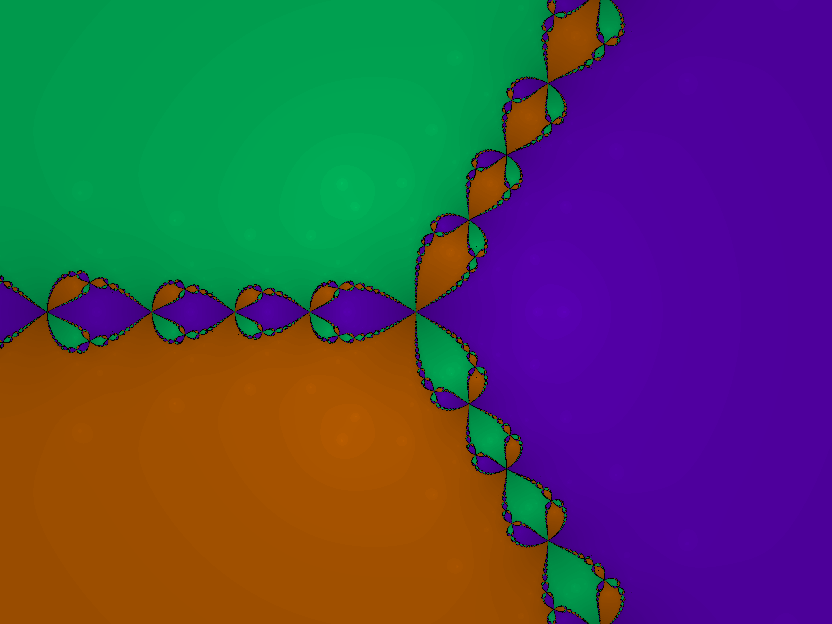
\includegraphics[width=0.95\textwidth]{compdyn01.png}
  \caption{Convergence diagram for $z^3-1$}
\end{figure}

We have many different stable behaviours of this dynamical system, but the boundary is very chaotic. For example, if we consider $p(z) = z^4-2z^2+9$, note that if $z \in \R$, then $f(z) \in \R$. However, the four roots of $p$ are all complex, and so Newton's method will fail to work for $z_0 \in \R$, and this can be seen in the following image:
\begin{figure}[H]
  \centering
  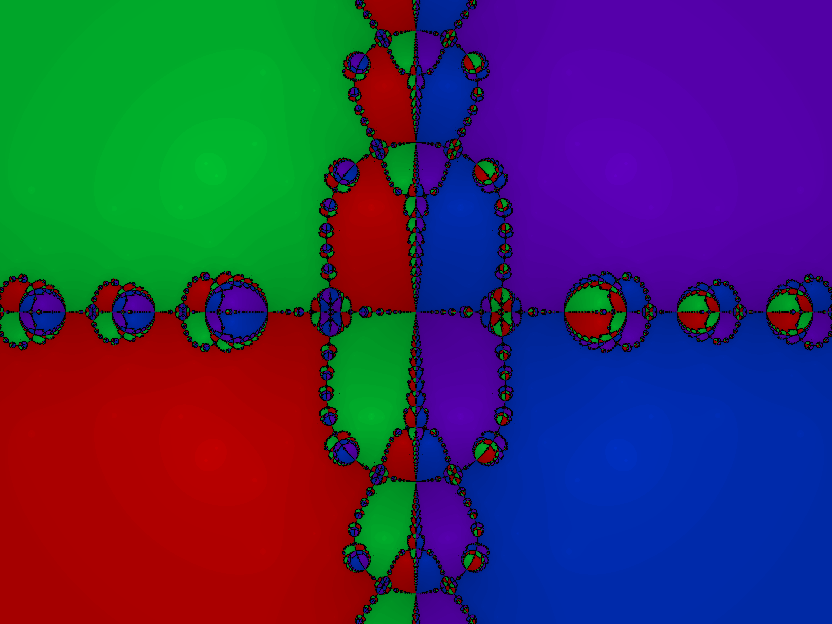
\includegraphics[width=0.95\textwidth]{compdyn02.png}
  \caption{Convergence diagram for $z^4-2z^2+9$}
\end{figure}

\subsection{Applications Motivation: Fixed Point Problems}
Gravitational Lensing: Suppose we have $n$ point masses in a plane perpendicular to the line of sight, and we are observing an object at the origin of this plane, identified with the complex plane. Call the points $z_1, \ldots, z_n$, with masses $\sigma_1, \ldots, \sigma_n$ respectively. Then the images of the object at the origin are the solutions to the \emph{lens equation} $z = \sum_{j=1}^n \frac{\sigma_j}{\bar{z} - \bar{z_j}}$. We see this for instance in the following image, courtesy of \texttt{Nasa}
\begin{figure}[H]
  \centering
  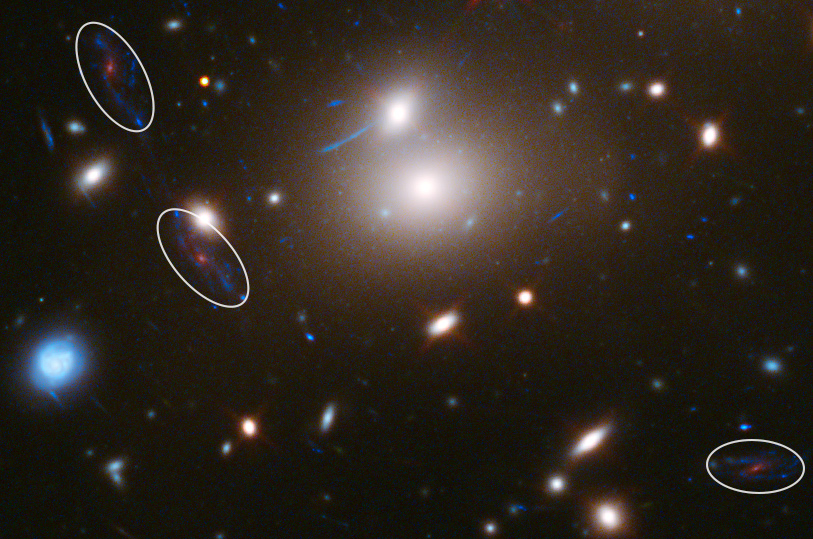
\includegraphics[width=0.95\textwidth]{compdyn03.jpg}
  \caption{The same galaxy appearing 3 times in an image captured by Hubble.}
\end{figure}

For example, if we have a point mass at the origin $n=1, z_1 = 0$. The lens equation gives us images of it at $z = \frac{\sigma_1}{\bar{z}}$, i.e. $\abs{z}^2 = \sigma_1$. The solution is a circle, known as an \emph{Einstein ring}.
\begin{figure}[H]
  \centering
  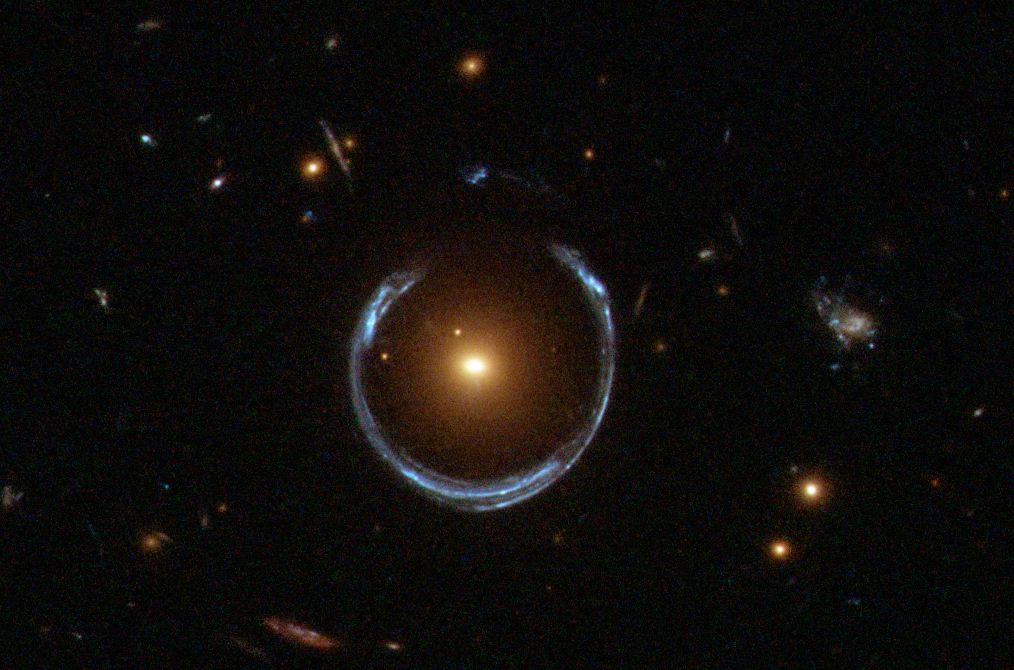
\includegraphics[width=0.95\textwidth]{compdyn04.jpg}
  \caption{An Einstein ring, captured by Hubble.}
\end{figure}

In general, we might want to ask how many images we will see for a give configuration, or perhaps a given number, of point masses.

Define $r(z) \coloneqq \sum_{j=1}^n \frac{\sigma_j}{z-z_j}$, and we are looking for solutions to $z = \overline{r(z)}$, i.e. fixed points of the (non-meromorphic) function $z \mapsto \overline{r(z)}$. These will be among the solutions of the (meromorphic) function $z\mapsto \overline{r(\overline{r(z)})} = r(r(z))$, of degree $n^2$. One can show that it suffices to bound the number of \emph{attracting} fixed points, which will be done in one of the main theorems of this course:

\begin{theorem}
Let $f(z)$ be a rational map of degree $d \geq 2$. Then $f$ has at most $2d-2$ attracting fixed points.
\end{theorem}

There are still open questions related to this application; for example, the following conjecture is still open despite its simplicity:
\begin{conjecture}[(Lee, Lerario, Lundberg)]
If $p$ is a polynomial of degree $n$, $q$ a polynomial of degree $m$, and $n>m$, then the number of solutions to $p(z) = \overline{q(z)}$ is bounded above by $2m(n-1)+n$.
\end{conjecture}

\subsection{Where We're Heading}
Define $f_c(z) \coloneqq z^2+c$, where $c \in \C$. \emph{The Mandelbrot Set} $M \coloneqq \{c \in \C : |f_c^n(0)|\nrightarrow\infty$ as $n\to\infty\}$.
\begin{figure}[H]
  \centering
  
\includegraphics[width=0.95\textwidth]{compdyn05.png}
  \caption{The Mandelbrot set, generated by me.}
\end{figure}

\section{Complex Basics}
\subsection{The Riemann Sphere}
The \emph{Riemann Sphere} $\hat{\C}$ is the one-point compactification of $\C$, given by adding a point at $\infty$. The basis of this topology around $\infty$ are the complements of the closed discs in $\C$.

\begin{definition}
A \emph{domain} in the Riemann sphere is any open connected subset of $\hat{\C}$.
\end{definition}
We can then think about \emph{maps of the Riemann sphere}, which are rational maps of the form $f(z) = \frac{p(z)}{q(z)}$, where $p, q$ are polynomials with no common roots. We define the \emph{degree} of $f$ to be the maximum of $\deg p, \deg q$.

\begin{definition}
We say that $f : \hat{\C} \to \hat{\C}$ is \emph{holomorphic at $\infty$} if $f(1/z)$ is meromorphic on a neighbourhood of 0.
\end{definition}

\begin{lemma}[Identity Principle]
Let $f: D \to D$ be a holomorphic, non-constant map on a domain $D$ in $\hat{\C}$. Then for any $w \in D, f^{-1}(w)$ is discrete. In particular, if $D = \hat{\C}$, then $f^{-1}(w)$ is finite.
\end{lemma}
\begin{proof}
First, composing with a M\"obius map, we may assume $w = 0$. By the principle of isolated zeros, $\forall z \in \hat{\C}$, there is some disc $D_z \ni z$ such that either $f \equiv 0$ on  on $D_z$ or $f$ is nonzero on $D_z \setminus \{z\}$.

Let $V \coloneqq \bigcup_{f = 0 \text{ on } D_z} D_z$, $W \coloneqq \bigcup_{f \neq 0 \text{ on } D_z} D_z$

Then $V \cup W = D$, these sets are open, and $V \cap W = \emptyset$. Since $D$ is connected, $V$ and $W$ cannot disconnect $D$, so one of $V$ and $W$ is empty. $f$ is nonconstant, so $V = \emptyset$, and so the zeros are discrete. As $\hat{\C}$ is compact, any discrete subset is finite.
\end{proof}

\begin{proposition}
Let $f: \hat{\C} \to \hat{\C}$ be a holomorphic, non-constant map. Then $f$ is a non-constant rational function; that is, there exist $a_1, \ldots, a_m, b_1, \ldots b_n \in \C$, and $c \in \C^{\times}$ such that:
\begin{align*}
f(z) = \frac{c(z-a_1)\ldots(z-a_m)}{(z-b_1)\ldots(z-b_n)}
\end{align*}
\end{proposition}

\begin{proof}
Replace by $\frac{1}{f}$ if necessary to assume $f(\infty) \in \C$. By the identity principle, $f^{-1}(\infty)$ is a finite subset of $\C$. Call it $\{b_1, \ldots, b_n\}$. Near each $b_j$, we have a local expansion of $f$ as $f(z) = \sum_{i=-k}^\infty a_{j,i}(z-b_j)^i$. Set $Q_j(z) = \sum_{i=-k}^{-1} a_{j,i}(z-b_j)^i$, each $Q_j$ is a rational function and $g \coloneqq f - (Q_1 + \ldots + Q_n)$ has only removable singularities. So $g(\hat{\C}) \subseteq \C$. Since $\hat{\C}$ is compact, $g(\hat{\C})$ is a compact, proper, open subset of $\C$ $\contr$ (by Heine-Borel). Therefore $g$ is constant, and $f$ is rational.
\end{proof}

\subsection{The Derivative at Infinity}
Caution: there is not a globally well defined notion of a derivative of $f:\hat{\C} \to \hat{\C}$, since we can change coordinates in many different ways. However, if $f(\infty) = \infty$, then we do, as the local derivative is independent of choice of coordinates. In this case, we define $f'(\infty)$ to be the derivative at 0 of $\frac{1}{f(1/z)}$.

\subsection{Uniformizations}
We say a group $\Gamma$ acts \emph{properly discontinuously} on a set if all points $p$ have a neighbourhood $N \ni p$ with $g(N) \cap h(N) = \emptyset$ for all $g \neq h \in \Gamma$

\begin{theorem}[Uniformization in $\hat{C}$]
  Let $U$ be a domain in $\hat{C}$. Then the universal cover $\tilde{U}$ of $U$ is either $\hat{\C}$, $\C$, or $\D$, and $U \simeq \tilde{U}/\Gamma$ for some subgroup $\Gamma \leq \Aut(\tilde{U})$ which acts properly discontinuously.
\end{theorem}

We now consider the different cases:
\begin{itemize}
  \item Universal Cover $\hat{\C}$: $\Aut(\hat{C}) = \{$M\"obius transformations$\}$

  All M\"obius transformations have at least one fixed point. So if $\Gamma$ acts properly discontinuously on $\hat{C}$, $\Gamma$ must be $\{\id\}$, and as such $U = \tilde{U} = \hat{C}$.

  \item Universal Cover $\C$: $\Aut(\C) = \{$M\"obius transformations fixing $\infty\}$

  These transformations are the linear maps, i.e. $f(z) = az+b, a \neq 0$. If a non-identity map lies in $\Gamma$, then it has no fixed point, and hence $az+b=z$ has no solutions, i.e. $a=1, b \neq 0$. So $\Gamma$ consists of the translations, and we can identify $g \in \Gamma$ with $g(0) \in \C$.

  $\Gamma \leq \C$ consists of isolated points, so $\Gamma = \{\id\}, \angle{\omega}$ for some $\omega \in \C$, or a lattice $\Lambda$.

  These correspond respectively to $U \simeq \C, U \simeq \C^\times$, and a complex torus (which is not a subdomain of $\C$).

  \item Universal Cover $\D$: $\Aut(\D) = \left\{e^{\im\theta} \frac{z-\omega}{1-\bar{\omega}z} : \theta \in \R, \omega \in \D\right\}$.

  All the rest! Any domain which omits at least three points of $\hat{\C}$ has the disc as its universal cover. This gives a lot of different subgroups of $\Aut(\D)$ - we won't study which ones are possible in this course.
\end{itemize}

\begin{definition}
  We say a domain $U \subseteq \hat{C}$ is \emph{hyperbolic} if it has universal cover $\D$, or equivalently if it omits at least 3 points.
\end{definition}

If $U$ is a hyperbolic domain, then the covering maps $\tilde{U} \to U$ are holomorphic. So if $f:U \to V$ is a holomorphic map between hyperbolic domains, then its lifted map $g$ is also holomorphic. $g$ is also unique up to a choice of an element of $\Gamma_V$

\begin{theorem}[Picard Theorem]
  If $U$ is a hyperbolic domain, and $f : \C \to U$ is holomorphic, then $f$ is constant.
\end{theorem}
\begin{proof}
  The following diagram commutes:
  \begin{tikzcd}
    \C \arrow{d}{\id} \arrow{r}{g} & \D \arrow{d}{\pi_U} \\ \C \arrow{r}{f} & U
  \end{tikzcd}

  So $g$ is a holomorphic function from $\C$ to $\D$, so bounded, so constant by Liouville's theorem. Hence $f$ must also be constant.
\end{proof}

In fact, there are no non-constant holomorphic maps from $\hat{C}, \C, \C^\ast$ to any hyperbolic domain.

Recall that the hyperbolic (or Poincar\'e) distance between any two points on the disc is the infimum along smooth curves $\gamma : [a,b] \to \D$ which connect the two points of the length value:\[ \ell(\gamma) = \int_a^b \frac{2}{1-|\gamma(t)|^2}|\gamma'(t)| dt\]

Using the origin and automorphisms, one computes that the distance function is given by \[d(x,y) = \frac{\log(1+R)}{\log(1-R)}\] where $R = \left|\frac{y-x}{1-xy}\right|$.

\begin{definition}[Hyperbolic/Poincar\'e metric of a hyperbolic domain]
  Taking the covering map $\pi:\D\to U$ for $U$ a hyperbolic domain to be a local isometry, we define a unique metric on $U$ known as the hyperbolic/Poincar\'e metric on $U$.
\end{definition}

\begin{theorem}[Pick Theorem]
  The $f:U\to V$ be a holomorphic map of hyperbolic domains $U, V \subset \hat{\C}$ with Poincar\'e metrics $\rho_U, \rho_V$ respectively. Then for all $x, y \in U$:\[ \rho_V(f(x), f(y)) \leq \rho_U(x,y)\] with strict inequality unless $f$ lifts to an automorphism of $\D$.
\end{theorem}
\begin{proof}
  By definition of $\rho_U, \rho_V$, it suffices to prove this for $f: \D \to \D$. We want to show that \[\frac{\log(1+R')}{\log(1-R')} \leq \frac{\log(1+R)}{\log(1-R)}\] where
  \begin{align*}
    R &= \left|\frac{y-x}{1-\bar{x}y}\right|,\;\;\;  R' = \left|\frac{f(y)-f(x)}{1-\overline{f(x)}f(y)}\right|
  \end{align*}

  As $\frac{\log(1+x)}{\log(1-x)}$ is strictly increasing, it is sufficient to show $R' \leq R$. Define:
  \begin{align*}
    \sigma_1(z) = \frac{y-z}{1-\bar{y}z},\;\;\;\;\sigma_2(z) = \frac{f(y)-f(z)}{1-\overline{f(y)}f(z)}
  \end{align*}
  Then $\sigma_2 \circ f \circ \sigma_1^{-1} : \D \to \D$ fixes 0. So by Schwarz's lemma, $|\sigma_2 \circ f \circ \sigma_1^{-1}(z)| \leq \abs{z}$, i.e.
  \[
    \left|\frac{f(y)-f(x)}{1-\overline{f(y)}f(x)}\right| \leq \left|\frac{y-x}{1-\bar{y}x}\right|
  \]
by setting $\sigma_1^{-1}(z) = x$. The statement with strict inequality follows similarly.
\end{proof}

Thus all maps of hyperbolic domains are (weakly) contracting with respect to the hyperbolic metric. This is in contrast to the non-hyperbolic case, where we can have things like $f:\C \to \C, z \mapsto 2z$ which is expanding, or $g:\hat{C} \to \hat{C}, z\mapsto z+1$, which has expansion and contraction at the same time in different regions.

\section{What is a reasonable notion of stable/predictable behaviour under iteration?}

For example, take $f(z) = z^2$, so that $f^n(z) = z^{2^n}$. If $\abs{z} > 1$, then $|f^n(z)| = \abs{z}^{2^n} \to \infty$. On the other hand, if we start with a point inside the unit disc, then $|f^n(z)| \to 0$. This is a stable property - if $z$ goes off to $\infty$ or $0$ under iteration of $f$, then $z+\epsilon$ for $|\epsilon|$ small also goes off towards $\infty$ or 0 respectively.

In contrast, if $\abs{z}=1$, then we do not have this stable behaviour.

\begin{definition}
  Let $S, T$ be metric spaces and $f_n : S \to T$ a sequence of continuous maps. We say that $\{f_n\}$ \emph{converges locally uniformly} if for all compact $K \subset S$ and all $\epsilon >0$ there exists $N \in \N$ such that
  \[
    \sup_{z \in K} d_T(f_n(z), f_m(z)) < \epsilon
  \]
  for all $n, m \geq N$.

  We say that $\{f_n\}$ \emph{diverges locally uniformly} if for all compact $K \subset S$ and compact $K' \subset T$, we have $N \in \N$ such that $f_n(K) \cap K' = \emptyset$ for all $n \geq N$.
\end{definition}

\underline{Example:} Let $p(z) = a_dz^d + \ldots + a_0 \in \C[z]$ a polynomial, with sequence of iterates $\{p^n(z) : n \in \N\}$. If $\abs{z} \gg \max\{|a_d|, \ldots, |a_0|\}$, then $|p(z)| \approx |a_dz^d|$. So $|p^n(z)| \to \infty$ as $n \to \infty$. Considering $p:\hat{\C} \to \hat{\C}$, the sequence $\{p^n(z)\}$ converges locally uniformly on a neighbourhood of $\infty$.

Note that the definition of $S, T$ matter - if we consider $p:\C \to \C$ instead then the sequence of iterates $\{p^n(z)\}$ diverges locally uniformly on the complement of some large disc.

\begin{definition}
  A family $\mathcal{F}$ of continuous functions $f: S \to T$ is \emph{normal} if every sequence in $\mathcal{F}$ has a subsequence which is either locally uniformly convergent or locally uniformly divergent.
\end{definition}

\begin{lemma}
  Let $U, V$ be domains and $\mathcal{F}$ a normal family of holomorphic maps $U \to V$. Then any sequence $\{f_n\}$ in $\mathcal{F}$ has a subsequence which converges to a holomorphic limit $g: U \to \bar{V}$, where $\bar{V}$ is the closure of $V$ in the Riemann sphere.
\end{lemma}
\begin{proof}
  $\mathcal{F}$ is normal, so pass to a subsequence of holomorphic maps to assume locally uniform convergence or divergence.

  If $\{f_n\}$ converges locally uniformly, then $\bar{V}$ compact implies we have a limit function $g: U \to \bar{V}$, by taking $K = \{\text{pt}\}$ in the definition. By the Weierstrass uniform convergence theorem, this is holomorphic.

  If $\{f_n\}$ diverges locally uniformly, then for any compact $K \subset U$, we have some convergent subsequence $f_{n_K}(z) \to z_0 \in \partial V$ for any choice of $z \in K$. If $U, V$ are hyperbolic, then by Pick's theorem, all elements of $K$ converge to $z_0$, and so we have local uniform convergence to the constant function at $z_0$. If $U, V$ are not hyperbolic, we may shrink $U$ slightly to still contain $K$, but be hyperbolic $U_0$ with compact closure in $U$.
  By local divergence, we can remove points from $V$ and initial elements of the sequence $\{f_n\}$ to assume $V$ is hyperbolic.
\end{proof}

\underline{Example:} $f(z) = z^2$. $\mathcal{F} \coloneqq \{f^n(z) : n \in \N\}$.

$\hat{\C} \setminus \bar\D$ is a hyperbolic domain, and $f:\hat\C\setminus\bar\D\to\hat\C\setminus\bar\D$, and the iterates $\{f^n(z)|_{\hat\C\setminus\bar\D}\}$ converge locally uniformly to the constant map at $\infty$. Similarly, $\{f^n(z)|_\D\}$ converge locally uniformly to the constant map at 0.

These sets are maximal for these behaviours, i.e. $\{f^n\}$ is a normal family on $\D$ and on $\hat\C\setminus\bar\D$ but on no larger set. If $|z_0| = 1$, then we have for any neighbourhood of $z_0$, some points go to infinity and some go to zero, and so there can be no holomorphic limit of iterates on any neighbourhood of $z_0$.

\section{A More Useful Criterion for Normality}
\textbf{Definition.} A family $\mathcal{F}$ of continuous functions $S \to T$ is \emph{equicontinuous} if, for all $\epsilon > 0$ there is $\delta >0$ such that, for all $f \in \mathcal{F}$ and all $s, t \in S$:
\[d_S(s,t) < \delta \implies d_T(f(s), f(t)) < \epsilon\]

\begin{theorem}[Arzel\`a-Ascoli in $\hat\C$]
  A family $\mathcal{F}: S \to T$ of continuous maps of domains $S, T \subset \hat\C$ has the property that all sequences have a locally uniformly convergent subsequence if and only if the following are both satisfied:
  \begin{itemize}
    \item $\mathcal{F}$ is equicontinuous on any compact subset of $S$, and
    \item For all $z \in S, \{f(z):f \in \mathcal{F}\}$ lies in a compact subset of $T$.
  \end{itemize}
\end{theorem}
\begin{proof}
  The forwards direction is left as an exercise.

  For the reverse direction, since $S, T \subseteq \hat\C$, we can fix a countable dense subset $\{z_k\}$ of $S$. Fix a sequence $\{f_n\}$ of elements of $\mathcal{F}$. We can find a set of indices $\{n_{ij}\}$ such that:
  \begin{align*}
    &n_{11} < n_{12} < n_{13} < \ldots < n_{1j} < \ldots\\
    &n_{21} < n_{22} < n_{23} < \ldots < n_{2j} < \ldots\\
    &\;\;\;\vdots\\
    &n_{i1} < n_{i2} < n_{i3} < \ldots < n_{ij} < \ldots\\
  \end{align*}
  so that each row is contained in the previous as a subsequence, and $\lim\limits_{j \to \infty} f_{n_{kj}}(z_k)$ exists for each $k$.

  The diagonal sequence $g_k \coloneqq f_{n_{kk}}$ is strictly increasing in index, and for each $k$, eventually contained in the $k\th$ row. So $g_k$ converges at each $z_k$.

  Consider now $K$, a compact subset of $S$. Given $\epsilon > 0$ there is $\delta >0$ such that, for all $x,y \in K$ and all $g_k$, $d_S(x, y) < \delta \implies d_T(g_k(x), g_k(y)) < \epsilon/3$.

  Cover $K$ by finitely many $\delta/2$ diameter neighbourhoods, selecting some $z_k$ for each of these neighbourhoods.

  Given $z \in K$, we have some $z_k$ with $\delta$, and there are only finitely many $z_k$ in this set, so in fact we can find $N$ such that $n, m > N$ implies $d_T(g_n(z_k), g_m(z_k)) < \frac{\epsilon}{3}$.

  So we have:
  \begin{align*}
    d_T(g_n(z), g_m(z)) &\leq d_T(g_n(z), g_m(z_k)) + d_T(g_n(z_k), g_m(z_k)) + d_T(g_m(z_k), g_m(z))\\
    &< \epsilon/3 + \epsilon/3 + \epsilon/3\\
    &= \epsilon
  \end{align*}
  Since this holds for all $z \in K$, we have locally uniform convergence as claimed.
\end{proof}
\addtocounter{theorem}{-1}
\begin{corollary}
  If $T$ is compact, a family of continuous maps from $S$ to $T$ is normal if and only if it is equicontinuous on compact subsets.
\end{corollary}

This brings us to the critical takeaway applicable to dynamics:
\begin{theorem}[Montel's theorem]
  Let $U, V$ be domains with $V$ hyperbolic. Then the family of holomorphic maps from $U$ to $V$ forms a normal family.
\end{theorem}
\begin{proof}
  Suppose first that $U$ is hyperbolic. By Pick's theorem, the family is equicontinuous.

  If $\exists x \in U$ such that $\{f(x) : f \in \mathcal{F}\}$ is in some compact $K \subseteq V$, then again by Pick's theorem, the same is true for all points in $U$. So by Arzel\`a-Ascoli, we have a normal family.

  Otherwise, we can fix $x \in U, y \in V$, and an infinite sequence $\{f_n\}\subseteq \mathcal{F}$ such that $\rho_V(f_n(x), y) \to \infty$ as $n \to \infty$. Fix compact $K \subseteq U, K'\subseteq V$, noting that $\rho_U(x, K), \rho_V(y, K')$ are finite, we have by Pick's theorem that $f_n(K) \cap K' = \emptyset$ for all $n$ sufficiently large. So this sequence diverges locally uniformly, and again we have a normal family.

  In the case where $U$ is not hyperbolic, then $\mathcal{F}$ consists of constant maps.

  If there is a subsequence with images in a compact set, then we have a locally uniformly convergent subsequence.

  If not, then only finitely many of these maps have image in any compact set - we have locally uniform divergence.
\end{proof}

\underline{Example:} $f(z) = z^2$. We've seen that $\{f^n(z) : n \in \N\}$ form a normal family on $\D$ and $\hat\C\setminus\bar\D$, by manual computation. But since $f^n(\D) \subseteq \D, f^n(\hat\C\setminus\bar\D)\subseteq\hat\C\setminus\bar\D$, the iterates of $f$ must form a normal family on these domains because the image spaces are hyperbolic.

More generally, if $U \subseteq \hat\C$ is a hyperbolic domain, either $\{f^n(U) : n \in \N\}$ covers all but at most 2 points of $\hat\C$, or the iterates of $f$ form a normal family on $U$.

\section{Degree and Ramification}
\begin{definition}
  A continuous map $f:U \to V$ of topological spaces is \emph{proper} if for all $K \subset V$, $f^{-1}(K)$ is compact in $U$.
\end{definition}
\addtocounter{theorem}{-1}
\begin{lemma}
  Let $f:U\to V$ be continuous. If $U$ is compact and $V$ is Hausdorff, then $f$ is proper.
\end{lemma}
\begin{proof}
  Let $K \subseteq V$ be compact. $V$ is Hausdorff $\implies$ $K$ is closed, so $V \setminus K$ is open $\implies f^{-1}(V\setminus K)$ is open (as $f$ is continuous). So $f^{-1}(K) = U \setminus f^{-1}(V\setminus K)$ is closed, and so compact as it is a closed subset of a compact set. So $f$ is proper.
\end{proof}

Recall from complex analysis the concept of local degree/ramification: if $f$ is holomorphic on a neighbourhood of $z_0$, with $f(z_0) = w_0$, then locally we have an expansion\[f(z) = w_0 + (z-z_0)^eg(z-z_0)\] where $g(z-z_0)$ is nonzero at $z_0$, and holomorphic on a neighbourhood of $z_0$. Then $e$ is the local degree/ramification index at $z_0$. If $e > 1$, then $z_0$ is said to be critical.

Let $U, V$ be domains in $\hat\C$.
\addtocounter{theorem}{-1}
\begin{proposition}
  If $f:U \to V$ is a proper holomorphic map, then $f$ has a well defined degree on $U$, equal to\[\sum_{z \in U: f(z) = w} e_z\] for any $w \in V$, where $e_z$ is the ramification index of $f$ at $z$.
\end{proposition}
Note that this is independent of $w$, and by Lemma \textbf{5.1}, all rational maps have well-defined degree!
\addtocounter{theorem}{-1}
\begin{theorem}[Riemann-Hurwitz]
  Let $f:U \to V$ be proper of degree $d$. Then\[\chi(U) = d\chi(V) - \sum_{p\in V}(e_p-1)\] where $e_p$ is the ramification index of $f$ at $p$ and $\chi$ is the Euler characteristic.
\end{theorem}
We will take both of these theorems for granted - they follow immediately from the corresponding statements for compact sets.

\begin{corollary}
  Any degree $d$ rational function $f$ has $2d-2$ critical points, counting multiplicity.
\end{corollary}
\begin{proof}
  $\chi(\hat\C) = 2$, and use Riemann-Hurwitz.
\end{proof}
\begin{corollary}
  If $U, V$ have $\chi(U) = \chi(V) = 0$, (e.g. annuli, punctured discs), then any proper holomorphic $f:U \to V$ is unramified.
\end{corollary}

\section{Julia Sets}
\begin{definition}[Fatou Set, Julia Set]
  Let $f$ be a nonconstant rational map. The \emph{Fatou set} of $f$ is:
  \[F(f) \coloneqq \{x \in \hat\C : \exists \text{ a neighbourhood } U \ni z\text{ on which }\{f^n|_U(z)\}\text{ form a normal family}\}\]

  The \emph{Julia set} of $f$ is $J(f) \coloneqq \hat\C\setminus F(f)$.
\end{definition}
Intuitively, $F(f)$ is the stable locus of $f$, and $J(f)$ is the chaotic or unstable locus of $f$.

For example, take $f(z) = \lambda z$ for $\lambda = e^{2\pi\im\theta}$ for some $\theta \in \R\setminus \Q$. Then $\{f^n(z)\}$ forms a normal family on any disc centered at $0$, because $\{f^n|_{\text{disc}}\}$ is a family of self-maps of hyperbolic domains, so we can use Montel's theorem. Note that $f^n(z)$ doesn't converge to any point, but it does have convergent subsequences.

\begin{figure}[H]
  \centering
  \begin{tikzpicture}
    \draw (2,0)--(2,4);
    \draw (0,2)--(4,2);
    \draw[blue] (2,2) circle (1);
    \node[circle, draw, fill, minimum size=1pt, inner sep=0pt, label={[shift={(0.1,-0.1)}]$\im$}] at (2,3) {};
    \node[circle, draw, fill, minimum size=1pt, inner sep=0pt, label={[shift={(0.2,-0.5)}]$-\im$}] at (2,1) {};
    \node[circle, draw, fill, minimum size=1pt, inner sep=0pt, label={[shift={(0.1,-0.1)}]$1$}] at (3,2) {};
    \node[circle, draw, fill, minimum size=1pt, inner sep=0pt, label={[shift={(-0.3,-0.1)}]$-1$}] at (1,2) {};
    \node[circle, draw, burgundy, fill, minimum size=1pt, inner sep=0pt, label={[shift={(0.1,-0.1)}]\color{burgundy}$z$}] at (2.8,2.6) {};
    \draw[dashed, burgundy] (2.8,2.6) circle (0.3) node[burgundy, label={[shift={(0.5,-0.3)}]\color{burgundy}$U$}] {};
  \end{tikzpicture}
\end{figure}
From now on in the course, we will usually only consider rational maps of degree at least 2. In the case of M\"obius transformations, the Fatou and Julia sets can be explicitly calculated - see example sheet 1.

\subsection{Basic Properties of J(F)}
It immediately follows from the definition that $F(f)$ is open, and so $J(F)$ is closed and compact in $\hat{\C}$.

\begin{lemma}
  The Fatou and Julia sets of $f$ are totally invariant under $f$. That is, $f(J(f)) = J(f) = f^{-1}(J(f))$, and similarly for $F(f)$.
\end{lemma}
\begin{proof}
  It suffices to show that $f^{-1}(F(f)) = F(f)$, and so to prove that, for any open $U \subseteq \hat\C$, a sequence of iterates $f^{n_k}(z)$ converges uniformly on compact subsets of $U$ if and only if $f^{n_k+1}(z)$ converges uniformly on compact subsets of $f^{-1}(U)$.

  We have:
  \[\sup_{z \in K}d(f^{n_j+1}(z), f^{n_k+1}(z)) = \sup_{w\in f(K)}d(f^{n_j}(w), f^{n_k}(w))\]

  Since $f$ is proper and continuous, preimages and images of compact sets are compact, and so we have the desired equivalence.
\end{proof}
This tells us why we get self similarity in Julia sets: if $z \in J(f)$ and $f'(z)\neq 0$, then there is a neighbourhood $N$ of $z$ such that $f:N \to f(N)$ is a conformal equivalence. Since $N \cap J(f) \xmapsto{f} f(N)\cap J(f)$, we have self-similarity.

\begin{lemma}
  $J(f) = J(f^n)$ for any iterate $f^n$ of $f$, and similarly for the Fatou set.
\end{lemma}
\begin{lemma}
  Let $f$ be a rational map and $\mu$ a M\"obius transformation, we define $g \coloneqq \mu \circ f \circ \mu^{-1}$. Then $\mu(J(f)) = J(g)$.
\end{lemma}
The proofs of these are exercises on example sheet 1.

\subsection{Conjugation and Dynamics}
In general, if $\mu$ is a M\"obius map, and $f$ is rational, with $g \coloneqq \mu\circ f\circ\mu^{-1}$, then \mbox{$g^n = \mu\circ f^n \circ \mu^{-1}$.}

As an example, let $f$ be a rational map of degree 2 with two fixed critical points. If $\infty$ is fixed, and $\infty$ maps to itself with degree 2, then we know $\infty$ has no other preimages, and we have a polynomial of degree 2. Let's conjugate by $\mu$, a M\"obius map taking one of the fixed critical points to $\infty$, and the other to 0.\footnote{Notice that being fixed and critical are conjugation invariant}

So we are conjugate to a degree 2 polynomial with 0 fixed and critical, i.e. $f(z) = az^2$. Conjugating again by $\mu(z) = az$, which doesn't change 0 or $\infty$, we have a map conjugate to $g(z) = z^2$. This has the unit circle as its Julia set.

Therefore $f$'s Julia set is a M\"obius image of the unit circle, i.e. a circle.

\begin{theorem}
  Let $z \in J(f)$ and $U$ be an open neighbourhood of $z$. Then the union $V \coloneqq \bigcup f^n(U)$ of forward images of $U$ contains all but at most two points of the Riemann sphere, both of which are critical points in the Fatou set.
\end{theorem}
\begin{proof}
  If $\{f^n|_U\}$ omit at least 3 points of $\hat\C$, then Montel's theorem tells us we have a normal family on $U$, and so $U \subseteq F(f)$. But $U \cap J(f)\neq \emptyset \contr$.

  If $\bigcup f^n(U)$ misses any points, then we want to show they are Fatou and critical. Without loss of generality, assume these points are in $\{0, \infty\}$. Since $f(V) \subseteq V$, no preimage of $0$ or $\infty$ lies in $V$.

  So the only possible behaviours are:
  \begin{enumerate}
    \item $0\mapsto 0, \infty \mapsto \infty$, both with degree $d = \deg f \geq 2$
    \item $0\mapsto \infty, \infty \mapsto 0$, both with degree $d$
    \item $\infty \mapsto \infty$ with degree $d$
    \item No points in this set.
  \end{enumerate}
  Hence all points in the set are critical, as they are images of ramification degree $d > 1$.

  In case 1, $f(z) = az^d$, conjugate to $z^d$, with 0, $\infty$ Fatou.

  In case 2, $f(z) = \frac{a}{z^d}$, conjugate to $z^{-d}$, with Julia set a circle again, so 0, $\infty$ Fatou.

  In case 3, $f(z)$ is a polynomial map, and so $\infty$ is Fatou.
\end{proof}
\begin{corollary}
  If the Julia set contains an interior point, then $J(f) = \hat\C$.
\end{corollary}
\begin{proof}
  By the previous theorem and forward invariance of the Julia set, if $U$ is open and contained in $J(f)$, then $\bigcup f^n(U) \subseteq J(f)$ contains all but at most two points of $\hat\C$. But $J(f)$ is closed, hence $J(f) = \hat\C$.
\end{proof}
The Julia set is the smallest closed totally invariant set in $\hat\C$ containing at least 3 points.

Note that $J(f) = \hat\C$ can happen, but not with polynomial maps. For instance, take $f(z) = \frac{1}{1-2z^2}$ - by the end of the course we'll be able to prove this function is chaotic everywhere.

On the other hand, we will show soon that $J(f) \neq \emptyset$.

\section{Cycles and Multipliers}
\begin{definition}
  Let $z_0 \in \hat\C$. We say that $z_0$ is \emph{periodic} or in a \emph{periodic cycle} for $f$ if $f^m(z_0) = z_0$ for some $m \in \N$. The minimal such $m$ is the period of the cycle. If $z_0$ has period $m$, then the derivative
  \[\lambda \coloneqq (f^m)'(z_0) = \prod_{i=0}^{m-1}f'(f^i(z_0))\]
  is called the \emph{multiplier} of the cycle.
\end{definition}
\underline{Example:} Take $p(z) = a_dz^d + \ldots + a_0$ a polynomial, so that $p(\infty) = \infty.$ Then $\infty$ is in a cycle of period 1. By example sheet 1, $p'(\infty) = \lim\limits_{z\to\infty}\frac{1}{p'(z)} = 0$. Hence $\infty$ is a fixed point of multiplier zero for any polynomial.

We classify periodic cycles according to their multiplier:
\begin{definition}
  Let $z_0$ be a point of period $m$ for $f$ with multiplier $\lambda$. Then we say $z_0$ is:
  \begin{itemize}
    \item \emph{superattracting} if $\lambda = 0$
    \item \emph{attracting} if $\abs{\lambda} < 1$
    \item \emph{indifferent} if $\abs{\lambda} = 1$
    \item \emph{repelling} if $\abs{\lambda} > 1$
  \end{itemize}
\end{definition}
Note that superattracting $\implies$ attracting.

If $g = \mu \circ f \circ \mu^{-1}$ for $\mu$ a M\"obius map, and $z_0$ has period $m$ for $f$ with multiplier $\lambda$, then $\mu(z_0)$ has period $m$ for $g$, again with multiplier $\lambda$.

\begin{definition}
  Suppose $C \coloneqq \{z_0, \ldots, z_{m-1}\}$ is an attracting orbit of period $m$. Then the \emph{basin of attraction} for the cycle $C$ is the set:
  \[\mathcal{A} \coloneqq \{z \in \hat\C:\lim_{n\to\infty}f^{nm}(z) \in C\}\]
\end{definition}
For example, take $f(z) = z^2, f'(z) = 2z$. Then if $z$ is a periodic point with period $m$, then $z = z^{2^m}$. These points are:
\begin{itemize}
  \item 0
  \item $\infty$
  \item Roots of unity of the form $z^{2^m-1} = 1$
\end{itemize}
These points respectively have multipliers:
\begin{itemize}
  \item $\lambda = 2\cdot 0=0$, and the basin of attraction is $\abs{z} < 1$.
  \item $\lambda = \lim\limits_{z\to \infty} \frac{1}{2z} = 0$, and the basin of attraction is $\abs{z} > 1$.
  \item $\abs{\lambda} = 2\abs{z} = 2$, so these are repelling.
\end{itemize}
\begin{theorem}
  Every attracting basin is contained in the Fatou set. Any repelling periodic point is contained in the Julia set.
\end{theorem}
\begin{proof}
  Since $J(f) = J(f^m)$ for $m \in \N$, we may assume that $z_0$ is a fixed point of $f$ with multiplier $\lambda$. Suppose that $\abs{\lambda} < 1$. Then locally, by Taylor's theorem, we have $\abs{f(z)-z_0} \leq c\abs{z-z_0}$ for any constant $\abs{\lambda}<c<1$. So we have uniform convergence of the iterates on compact subsets on a neighbourhood of $z_0$ to the constant function $z \mapsto z_0$. So $z_0 \in F(f)$ as claimed.

  If $z \in J(f)$, with $\lim\limits_{n\to\infty} f^n(z) = z_1$ say, then $z_1 \in J(f)$. But by above, $z_1 \in F(f)\contr$. Hence the attracting basin of an attracting point is also Fatou.

  Suppose $\abs{\lambda} > 1$. The derivative at $z_0$ of the iterates $f^k(z)$ is $\lambda^k \to \infty$ as $k \to \infty$. So there is no equicontinuity of $\{f^k\}$ on any neighbourhood of $z_0$, and so by Arzel\`a-Ascoli, $\{f^k\}$ is not normal on a neighbourhood of $z_0$. Hence $z_0 \in J(f)$.
\end{proof}

The derivative at fixed points is a local property, but it turns out there is still some global constraints on the multipliers of fixed points.
\begin{definition}
  Let $z_0$ be a fixed point of a rational map $f$ of degree $d$. The residue index of $f$ at $z_0$ is
  \[ i_f(z_0) \coloneqq \frac{1}{2\pi\im}\int_\gamma \frac{dz}{z-f(z)}\]
  where $\gamma$ is any small positively oriented loop around $z_0$.
\end{definition}
Note: a degree $d$ map has $d+1$ fixed points.
\begin{lemma}
  Let $\lambda$ be the multiplier of a fixed point $z_0$ of $f$. If $\lambda \neq 1$, then
  \[i_f(z_0) = \frac{1}{1-\lambda}\]
\end{lemma}
\begin{proof}
  Without loss of generality, assume that $z_0 = 0$ or $z_0 = \infty$, after noticing that both the residue and the multiplier are invariant under conjugation by a translation.

  If $z_0 = 0$, then $f(z) = \lambda z + a_2z^2 + a_3z^3 + \ldots$ near $z_0=0$. Since $\lambda \neq 1$, we have
  \begin{align*}
    z-f(z) &= (1-\lambda)z(1+b_1z+b_2z^2+\ldots)\\
    \implies \frac{1}{z-f(z)} &= \frac{1}{(1-\lambda)z}\frac{1}{1+b_1z+b_2z^2+\ldots}\\
    &= \frac{1}{(1-\lambda)z}(1+c_1z+c_2z^2+\ldots)\\
    &= \frac{1}{(1-\lambda)z} + g(z)
  \end{align*}
  where $g(z)$ is holomorphic. Integrating both sides causes the $g(z)$ to disappear, and so by the residue theorem we have the result.

  If $z_0 = \infty$, a similar computation works.
\end{proof}
On example sheet 1, there is an exercise to show that the residue index is conjugation invariant by any M\"obius map. Note that this lemma deals with every case except for when $\lambda = 1$.

\begin{theorem}[Holomorphic Lefschetz on the Riemann Sphere]
  Let $f:\hat\C \to \hat\C$ be a rational map of degree at least $2$. Then
  \[ \sum_{z=f(z)} i_f(z) = 1\]
\end{theorem}
\begin{proof}
  Assume without loss of generality that $\infty$ is not a fixed point. Let $C_R$ denote the circle of radius $R$ about $0$, positively oriented, and suppose that it is large enough to strictly contain all the fixed points of $f$. Then with $w = \frac{1}{z}$:
  \begin{align*}
    \int_{C_R} \frac{dz}{z-f(z)} = \int_{-C_{1/R}}\frac{-dw}{w^2\left(\frac{1}{w}-f(\frac{1}{w})\right)} = \int_{C_{1/R}}\frac{dw}{w\left(1-wf(\frac{1}{w})\right)}
  \end{align*}

  The nonzero poles of the integral are reciprocals of the fixed points of $f$, which by construction lie outside $C_{1/R}$. So, by the residue theorem, :
  \begin{align*}
    \sum_{z=f(z)}i_f(z) = \frac{1}{2\pi\im}\int_{C_R}\frac{dz}{z-f(z)} = \substack{\text{Res}\\w=0}\left[\frac{1}{w\left(1-wf(\frac{1}{w})\right)}\right] = 1
  \end{align*}
\end{proof}
\subsection{Structure of the Julia Set}
We have shown already that $J(f)$ is compact, and has no interior points unless $J(f) = \hat\C$. In this section we will show some other structural properties, starting with the following corollary of \textbf{7.7}
\begin{corollary}
  A rational map $f$ of degree $d \geq 2$ has a nonempty Julia set.
\end{corollary}
\begin{proof}
  Suppose that $J(f)=\emptyset$, and $f$ is of degree $d\geq 2$, so that $f$ has $d+1$ fixed points, counting with multiplicity.

  Since any repelling fixed point lies in $J(f)$, we can assume that $|\lambda| \leq 1$ for all fixed points of $f$. Suppose first that no fixed point has multiplier 1. Then the derivative of $f(z)-z$ is $f'(z)-1$, so we have all of the $d+1$ fixed points of $f$ distinct, as $f'(z)\neq 1$. Then all multipliers lie in $\bar{\D}$, and the map $x \mapsto \frac{1}{1-x}$, so that $\lambda(z) \mapsto i_f(z)$, is a M\"obius transformation taking $\bar{\D}$ to $\{z : \Re(z) \geq \frac{1}{2}\}$. So the sum of the $i_f(z)$ has real part $\geq \frac{d+1}{2} > 1$, violating \textbf{7.7}.

  Suppose now that $\lambda = 1$ for some fixed point $f(z_0) = z_0$ - \textsc{wlog}, move it to 0. Then locally, $f(z) = z + a_kz^k + \ldots$, $a_k \neq 0$, and so:
  \[f^n(z) = z+na_k z^k + \ldots\]
  Hence the $k\th$ derivative of $f^n$ at $z_0$ tends to $\infty$ as $n \to \infty$, and so we don't have normality on any neighbourhood of $z_0$, and so $z_0 \in J(f)$.
\end{proof}

In fact, we have proved something slightly stronger. We've proved that:
\begin{enumerate}
  \item Any periodic cycle with $\lambda^k = 1$ for some $k\in \N$ is contained in $J(f)$.

  If $\lambda$ is a multiplier with $\lambda^k = 1$ for some $k \in \N$, $f^k$ has a periodic cycle with $\lambda = 1$, and so the cycle is contained in $J(f^k)$. Since $J(f) = J(f^k)$, any such cycle is contained in $J(f)$.
  \item $J(f)$ is infinite.

  We produced a fixed point $z_0$ with $\abs{\lambda} \geq 1$ and $z_0 \in J(f)$. Consider $S = \bigcup\limits_{n \in \N\cup\{0\}}f^{-n}(z_0)\subseteq J(f)$. If this is finite, then since all elements' preimages are still in the set, $f$ must act as a bijection on $S$. Since $f(z_0) = z_0$, $z_0$ is its only preimage, so $f'(z_0) = 0, \contr$.
\end{enumerate}
\underline{Example:} $f(z) = z^2+\frac{1}{4}$. Consider the fixed points: $f(\infty) = \infty, f(1/2) = 1/2$. $\infty$ has multiplier 0, and is mapped to itself with degree $2$. $\frac{1}{2}$ has multiplier 1, so lies in $J(f)$, as do its infinitely many iterated preimages.

\begin{proposition}
  If $\mathcal{A}\subset \hat\C$ is the attracting basin of a periodic orbit for $f$. Then the Julia set $J(f)$ is the topological boundary $\partial \mathcal{A}$ of $\mathcal{A}$.
\end{proposition}
\begin{proof}
  Let $U$ be an open neighbourhood intersecting $J(f)$. Then we have already seen that $\bigcup_{n \in \N} f^{n}(U)$ contains all but at most 2 points of $\hat\C$, and so intersects $\mathcal{A}$, i.e., $f^n(U) \cap \mathcal{A} = \emptyset$ for some $n \in \N$.

  $U$ was arbitrary, and hence $J(f) \subseteq \bar{\mathcal{A}}$. Then $J(f) \cap \mathcal{A} = \emptyset \implies J(f)\subseteq \partial\mathcal{A}$.

  Now suppose that $z \in \partial \mathcal{A}$. If $U$ is a neighbourhood of $z$ on which the iterates form a normal family (i.e. $z \in F(f)$), then pick a convergent subsequence of $\{f^k\}$ converging to $g$, holomorphic on $U$. Then $g|_U$ on $U \cap \mathcal{A}$ takes one of a finite number of values, namely the elements of the cycle with $\mathcal{A}$ is attracting to. So $g$ must be constant as it is holomorphic. Hence $U \subseteq \mathcal{A}$, contradicting that $z \in \partial A$. Therefore $z \notin F(f)$, i.e. $z \in J(f)$. Hence $\partial \mathcal{A} \subseteq J(f)$.
\end{proof}
\underline{Example:} Consider again $f(z) = z^2$. Then, given $\alpha = \exp(2\pi\im \theta)\in J(f)$, the preimages of $\alpha$ are all the numbers which are a root of $z^{2^m} -\alpha = 0$ for some $m \in \N$, i.e. $\{\exp(2\pi\im \frac{\theta + k}{2^m}): m \in \N, 0\leq k<2^m\}$. These points provide a dense subset of $J(f)$, the unit circle.

\begin{corollary}
  For any rational map $f$ and $z_0 \in J(f)$, the set of preimages
  \[ \left\{ z: f^m(z) = z_0 \text{ for some } n\geq 0\right\}\]
  form a dense subset of $J(f)$.
\end{corollary}
\begin{proof}
  If we fix $z_0, z_1 \in J(f)$, if $z_1$ is not approximated by preimages of $z_0$, then there is some neighbourhood $U$ of $z_1$ whose forward images don't contain $z_0$. But these forward images contain all but at most 2 Fatou points of $\hat\C$, and in particular contain the Julia set, and hence $z_0\contr$.
\end{proof}
\begin{definition}
  A set is \emph{perfect} if it is closed with no isolated points, or equivalently is equal to its set of limit points.
\end{definition}
$J(f)$ is thus a perfect set: it is closed and infinite, so it contains at least one non-isolated point $z_0$. The preimages of $z_0$ form a dense non-isolated subset of the Julia set, so no point of $J(f)$ is isolated.

\section{Local Dynamics of Attractors}
Shr\"oder's equation: when is there a conformal change of variable $\phi$ so that $\phi(f(z)) = \lambda(\phi(z))$ on a neighbourhood of a fixed point $p$ for $f$, where $\lambda$ is the multiplier of that fixed point?

\begin{theorem}[Koenig's Linearization Theorem]
  Let $p$ be a fixed point of $f$ with multiplier $\lambda$ satisfying $|\lambda|\neq 0, 1$. Then there exists a local holomorphic change of coordinates $w = \phi(z)$ so that $\phi(p) = 0$ and $\phi\circ f\circ \phi^{-1}(w) = \lambda w$ for all $w$ in some neighbourhood $U$ of $p$, so that the diagram
  \begin{center}
    \begin{tikzcd}
      U \arrow{r}{f} \arrow{d}{\phi} & f(U) \arrow{d}{\phi}\\ \C \arrow{r}{\lambda}& \C
    \end{tikzcd}
  \end{center}
  commutes. This change of coordinates is unique up to multiplication by a constant.
\end{theorem}
\begin{proof}
  The idea is to prove that $\lim\limits_{n\to\infty} \frac{f^n(z)}{\lambda^n}$ exists as a holomorphic function on a neighbourhood of $p$, and then we're almost done.

  Conjugate to assume that $p=0$. Now suppose $|\lambda|<1$. Then there is a constant $c$ such that $c^2<|\lambda|<c<1$. By Taylor's theorem, there is $r >0$ such that, on $D(0, r)$, we have $|f(z)|\leq c|z|$. So for $z \in D(0,r)$ we have geometric convergence $|f^n(z)| \leq rc^n$. Again by Taylor, we have some constant $B$ such that $|f(z)-\lambda z| \leq B|z|^2$ on $D(0,r)$ (shrinking $r$ if necessarily). Hence for $z \in D(0,r)$:
  \[|f^{n+1}(z)-\lambda f^n(z)| \leq B|f^n(z)|^2 \leq B r^2c^{2n}\]
  \[\implies \left|\frac{f^{n+1}(z)}{\lambda^{n+1}} - \frac{f^n(z)}{\lambda^n}\right| \leq B\left(\frac{r^2}{|\lambda|}\right)\left(\frac{c^2}{|\lambda|}\right)^n \to 0 \text{ as } n \to \infty\]

  So $\frac{f^n(z)}{\lambda^n}$ converge uniformly on compact subsets of $D(0,r)$, to a holomorphic limit
  \[\phi(z) \coloneqq \lim_{n\to\infty} \frac{f^n(z)}{\lambda^n}\]
  We have $\phi(f(z)) = \lambda \phi(z)$, and $\phi'(0) = 1$ as $z \mapsto \frac{f^n(z)}{\lambda^n}$ has derivative 1 at $0$ for all $n$.

  So $\phi$ is conformal on a neighbourhood of $0$.

  To show that this is unique, suppose $\psi$ is another such. Then we have a commutative diagram:
  \begin{center}
    \begin{tikzcd}[
        row sep=4ex,
      ]
      V \arrow{r}{\lambda} \arrow{d}{\psi^{-1}} & \lambda \cdot V \arrow{d}{\psi^{-1}}\\
      U \arrow{r}{f} \arrow{d}{\phi} & f(U) \arrow{d}{\phi}\\
      \C \arrow{r}{\lambda} & \C
    \end{tikzcd}\hspace{2cm}
    \begin{tikzcd}[%
        row sep = 4ex,
      ]
      \makebox[\widthof{$\phi(\psi^{-1}(w))$}][r]{$w$} \arrow[mapsto]{r} \arrow[mapsto, shift left=7.5]{d} & \makebox[\widthof{$\lambda\phi(\psi^{-1}(w)) = \phi(\psi^{-1}(\lambda w))$}][l]{$\lambda w$} \arrow[mapsto, shift right=20]{d}\\
      \makebox[\widthof{$\phi(\psi^{-1}(w))$}][r]{$\psi^{-1}(w)$} \arrow[mapsto]{r} \arrow[mapsto, shift left=7.5]{d} & \makebox[\widthof{$\lambda\phi(\psi^{-1}(w)) = \phi(\psi^{-1}(\lambda w))$}][l]{$\psi^{-1}(\lambda w) = f(\psi^{-1}(w))$} \arrow[mapsto, shift right=20]{d}\\
      \phi(\psi^{-1}(w)) \arrow[mapsto]{r} & \lambda\phi(\psi^{-1}(w)) = \phi(\psi^{-1}(\lambda w))
    \end{tikzcd}
  \end{center}
  Hence $\lambda\phi(\psi^{-1}(w)) = \phi(\psi^{-1}(\lambda w))$. So $\phi\circ \psi^{-1}$ is conformal, on a neighbourhood of $0$, fixes 0, and commutes with $\lambda$. Taking a Taylor series,
  \begin{align*}
    \phi\circ \psi^{-1}: w &\mapsto a_1 w+ a_2w^2 + \ldots\\
    \lambda w &\mapsto a_1(\lambda w) + a_2(\lambda^2 w^2) +\ldots = \lambda(a_1 w + a_2 w^2 + \ldots)
  \end{align*}
  By uniqueness of Taylor series, $\lambda a_k = \lambda^k a_k$ for all $k \in \N$, and so, since $|\lambda| \neq 0,1$, $a_k = 0$ for $k \geq 2$. So $\phi\circ \psi^{-1}(w) = a_1 w$. Apply for $f^{-1}$ for the repelling case.
\end{proof}
\begin{corollary}
  Suppose $p$ is an attracting fixed point of $f$ with multiplier $\lambda \neq 0$ and basin of attraction $\mathcal{A}$. Then there is a holomorphic (not necessarily conformal) map $\phi:\mathcal{A}\to \C$ so that the following diagram commutes:
  \begin{center}
    \begin{tikzcd}
      \mathcal{A} \arrow{r}{f} \arrow{d}{\phi} &\mathcal{A} \arrow{d}{\phi}\\
      \C \arrow{r}{\lambda}& \C
    \end{tikzcd}
  \end{center}
  which is biholomorphic on a neighbourhood of $p$ and unique up to multiplication by a constant.
\end{corollary}
\begin{proof}
  Define by the previous theorem $\phi$ on a neighbourhood of $p$, $\phi(p) = 0, \phi(f(z))=\lambda \phi(z)$. Then for all $z \in \mathcal{A}$, there is by definition some $n \in \N$ such that $f^{n}(z) \in \dom \phi$. Thus:
  \[\phi(z) \coloneqq \lim_{n\to\infty} \frac{\phi(f^n(z))}{\lambda^n}\]
  satisfies the corollary.
\end{proof}
\begin{definition}
  A fixed point $p$ of $f$ is \emph{topologically attracting} if there is a neighbourhood $U$ of $p$ such that $\{f^n\}$ converges locally uniformly to the constant map $z \mapsto p$ on $U$.
\end{definition}
If $p$ is topologically attracting, then $p \notin J(f)$.

\begin{lemma}
  A fixed point $p$ is topologically attracting if and only if it is attracting, that is, if and only $|f'(p)|=|\lambda| < 1$.
\end{lemma}
\begin{proof}
  We've shown that attracting implies topologically attracting via Taylor's theorem. If $p$ is topologically attracting, then there is a disc $D(p,r)$ for $r>0$ and some iterate $f^n$ such that $f^n(D(0,r))\subsetneq D(0,r)$.

  Then Schwarz's lemma implies that $|(f^n)'(p)|=|\lambda|^n < 1$, so $|\lambda|<1$.
\end{proof}
\subsection{Generalizing to Period >1}
If $\{z_0, \ldots, z_{n-1}\}$ is an attracting cycle, so that $z_i$ is an attracting fixed point of $f^n$, each with attracting basing $\mathcal{A}_i$ (under $f^n$).

The $\mathcal{A}_i$ are permuted by $f$, so that $f(\mathcal{A}_i) = \mathcal{A}_{i+1}$ - this is an exercise on ES1.

Then we generalise to the commutative diagram
\begin{center}
  \begin{tikzcd}
    \mathcal{A}_0 \arrow{r}{f} \arrow{d}{\phi_0} & \mathcal{A}_1 \arrow{r}{f} \arrow{d}{\phi_1} & \ldots \arrow{r}{f} & \mathcal{A}_{n-1} \arrow{r}{f} \arrow{d}{\phi_{n-1}} & \mathcal{A}_0 \arrow{d}{\phi_0}\\
    \C \arrow{r}{\lambda_0} & \C \arrow{r}{\lambda_1} & \ldots \arrow{r}{\lambda_{n-2}} & \C \arrow{r}{\lambda_{n-1}} & \C
  \end{tikzcd}
\end{center}
where $\lambda_k = f'(z_k)$.

\begin{definition}
  The \emph{immediate basin} of an attracting cycle is the union of connected components of the Fatou set containing all cycle elements.
\end{definition}
Note that this is not iteration invariant. E.g. if we have a 3-cycle between Fatou components, then the immediate basin of a cycle $z_0\to z_1 \to z_2 \to z_0$ under $f$ will not be the same as the immediate basin of $z_0$ under $f^3$.

\begin{theorem}
  Suppose $f: \hat{\C}\to \hat{\C}$ has degree $d\geq 2$. Then every attracting fixed point of $f$ has a critical point in its immediate basin. Consequently, $f$ has at most $2d-2$ attracting cycles.
\end{theorem}
\begin{proof}
  A fixed attractor has connected immediate basin, so call it $U$. $U$ is hyperbolic since $J(f)$ is infinite, so we have
  \begin{center}
    \begin{tikzcd}
      \D \arrow{r}{F} \arrow{d}{\pi} & \D \arrow{d}{\pi}\\
      U \arrow{r}{f} & U
    \end{tikzcd}
  \end{center}
  If $U$ has no critical point, $f\circ \pi$ doesn't either, so is a covering map itself. So by universality there is $G:\D \to \D$ so that
  \begin{center}
    \begin{tikzcd}
      \D \arrow{d}{\pi} & \D \arrow{l}{G} \arrow{d}{\pi}\\
      U \arrow{r}{f} & U
    \end{tikzcd}
  \end{center}
  commutes, as $\D$ is the universal cover of $U$. Choosing the fixed point of $U$ to lift to 0, choose lifts $F, G$ to each fix 0. Then $G$ is an inverse to $F$, so $F$ is a disc automorphism, contradicting 0 being attracting.
\end{proof}

If $z_0 \mapsto z_1 \mapsto \ldots \mapsto z_{n-1} \mapsto z_0$ is an attracting cycle of period $n$ for $f$, then let $A_i$ be the immediate basin of $f^n$ for $z_i$. If $\bigcup_i A_i$ contains no critical point of $f$, since $f(A_i) = A_{i+1 \mod n}$ and $(f^n)'(z) = \prod_{i=0}^{n-1}f'(f^i(z_0))$, we see that there can be no critical points of $f^n$ in $A_i$ for any $i$, contradicting what we just proved.

So the immediate basin of every attracting cycle contains a critical point of $f$. $f$ has at most $2d-2$ critical points, and so we can only have $2d-2$ attracting cycles.

\begin{theorem}
  Suppose $f(0)=0$ is attracting for $f$, with multiplier $\lambda \neq 0$, immediate basin $\mathcal{A}_0$, and linearizing coordinate $\phi$ with local inverse $\psi : \D(0, \epsilon) \to \mathcal{A}_0$. Then $\psi$ extends by analytic continuation to a maximal open disc $\D(0, r)$, extends homeomorphically over the boundary circle $\partial \D(0, r)$, and the image $\psi(\partial \D(0, r)) \subset \mathcal{A}_0$ contains a critical point.
\end{theorem}
\underline{Example:} Take $f_c(z) = z^2+c$ for $c \in \C$.

We know that $f_c$ has a critical point at $\infty$ of multiplicity $2$. Since $2\cdot 2-2=2$, we have exactly one other critical point, which is at 0. By \textbf{8.6}, there is at most one attracting cycle other \mbox{than $\infty$.}

Suppose we have fixed point attractor: then $z_0$ fixed implies that $c = z_0 - z_0^2$, and $z_0$ attracting, since $\lambda =  f'(z_0) = 2z_0$, happens if and only if $|z_0| <\frac{1}{2}$. So the set of parameters $c$ with an attracting fixed point is the image of $\D(0, \frac{1}{2})$ under $z_0 \mapsto z_0-z_0^2$, i.e. the image of $\D$ under $\lambda \mapsto \frac{\lambda}{2} - \left(\frac{\lambda}{2}\right)^2$, a cardioid.

Suppose we have a period 2 attractor: then $(z_0^2+c)^2 +c = z_0$, and $z_0$ not fixed.
\[z_0^4+2cz_0^2-z_0 + c^2 + c = 0 \iff (z_0^2-z_0 + c)(z_0^2+z_0+c+1) = 0\]
The roots of the first factor are fixed, so we want the roots of $z_0^2+z_0+c+1$. So $c+1 = -z^2-z_0$. The multiplier for a period 2 point $z_0$ is \mbox{$\lambda = 4z_0(z_0^2+c)=4z_0(z_0^2-z_0^2-z_0-1) = 4z_0(-z_0-1) = 4(c+1)$.} Hence the parameters with a period 2 attractor is the image of $\D$ under $\lambda \mapsto \frac{\lambda}{4}-1$, i.e.  $\D(-1, \frac{1}{4})$.

\begin{figure}[H]
  \centering
  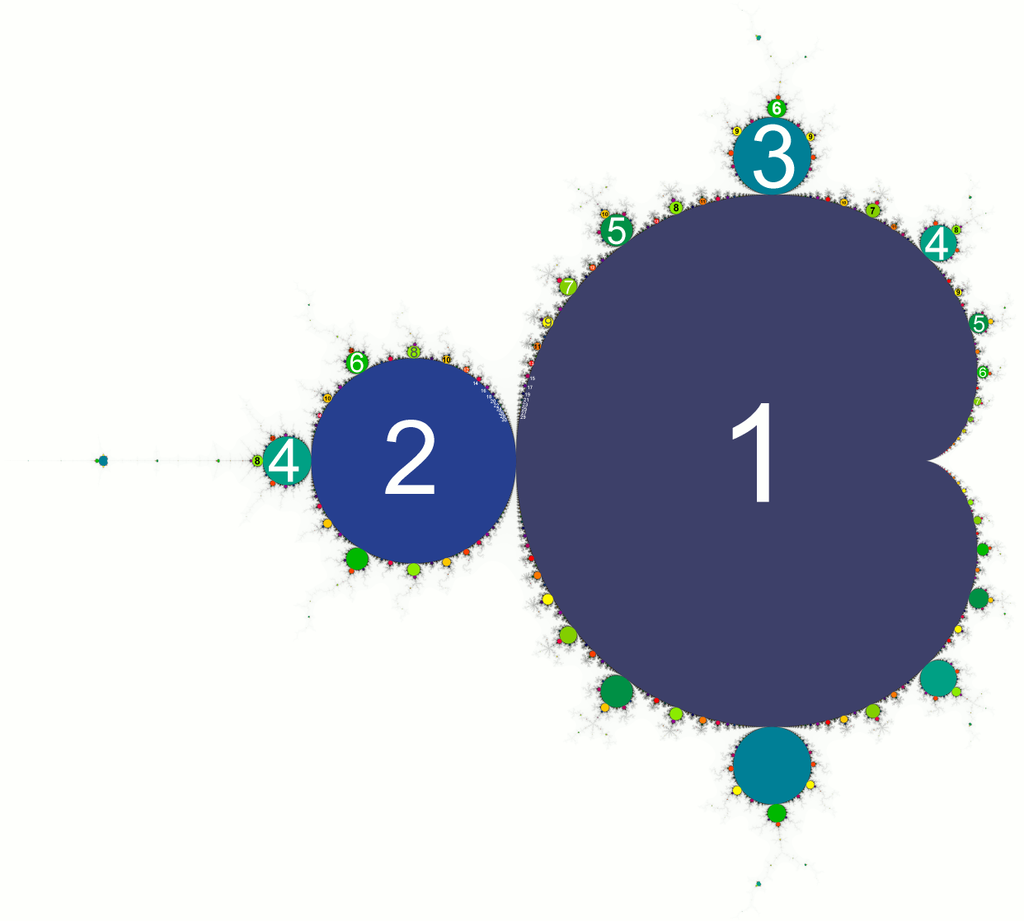
\includegraphics[width=0.95\textwidth]{compdyn06.png}
  \caption{Figure showing the locus of $c$ leading to attracting period $n$ points in $f_c$. Source: wikimedia commons}
\end{figure}

As a point of caution, note that attracting basins need not be connected. In fact, disconnected Julia sets have many components.

\begin{theorem}
  If a rational map $f$ has disconnected Julia set, then $J(f)$ has uncountably many connected components.
\end{theorem}
\begin{proof}
  Suppose $J(f)$ is not connected, so that $J(f) = J_0 \cup J_1$, two non-empty disjoint compact infinite subsets of $J(f)$. Given $z \in J(f)$, we assign a sequence of values $\{\beta_n(z)\}$ of 0s and 1s, with $\beta_n(z) = 0$ if $f^n(z) \in J_0$, and 1 otherwise. 2 points in the same connected components have the same sequence since $f$ is continuous. So $\beta: z\to \{(\beta_n)\}$ is a map from the connected components of $J(f)$ to $\{0,1\}^\N$.

  Let $(\beta_0(z), \ldots, \beta_k(z))$. be some finite piece of the sequence for fixed $z \in J(f)$. If we can show that there is $z' \in J(f)$ such that $\beta_i(z') = \beta_i(z)$ for all $0\leq i\leq k$, but there is $n > k$ such that $\beta_n(z') \neq \beta_n(z)$, then $\beta$ will have an uncountable image, and we will be done.

  Define $U_{z,k} \coloneqq \{w \in \hat\C: f^i(w) \notin J_{1-\beta_i(z)} \forall 0 \leq i \leq k\}$. Note that $U_{z,k}$ is open and contains the Fatou set for all $z, k$.

  Choose a constant subsequence $(\beta_{n_j}(z))$, say always taking the value $\beta_0(z)$. If $z' \in J(f)$ with $\beta_i(z') = \beta_i(z)$ for all $0 \leq i\leq k$, then $z' \in U_{z, k}$, and if $z' \in F(f), z' \in U_{z,k}$. If, for any $z'$ with $\beta_i(z) = \beta_i(z')$ for all $0\leq i\leq k$, then $\beta_n(z)=\beta_n(z')$ for all $n$, then $\beta_{n_j}(z) = \beta_{n_j}(z')$ for all $j$.

  I.e. $f^{n_j}(z') \in U_{z, n_j} = U_{z, 0}$. So $f^{n_j}|_{U_{z,k}} : U_{z,k} \to U_{z,0}$. Since $J_0, J_1$ are infinite, $U_{z,0}$ is hyperbolic, and so by Montel's theorem, we have a normal family, and $U_{z, k} \subseteq F(f) \contr.$

  Hence the image of $\beta$ is uncountable.
\end{proof}

\begin{theorem}[B\"ottcher 1904]
  Suppose $f(0) = 0$ is holomorphic, with local expansion
  \[f(z) = a_mz^m + a_{m+1}z^{m+1}+\ldots, m \geq 2\]
  Then there is a holomorphic local change of coordinate $\phi$ with $\phi(0) = 0$ so that $\phi(f(z)) = \phi(z)^m$. $\phi$ is unique up to multiplication by an $(m-1)\th[st]$ root of unity.
\end{theorem}
\begin{proof}
  This proof is similar to the proof of Koenig's theorem.

  Assume by conjugating with an $(m-1)\th[st]$ root $a_m$, say $\alpha$, that $a_m = 1$. So we write
  \[ f(z) = z^m(1+h(z))\]
  where $h$ is holomorphic on a neighbourhood of $0$, and $h(0) = 0$.

  We have a holomorphic logarithm $k(z)$ of $1+h(z)$ on a small neighbourhood of $0$, so $1+h(z) = e^{k(z)}$. By induction, we see that
  \[f^n(Z) = z^{m^n}e^{k_n(z)},\;\;k_n(z)\text{ holomorphic}\]
  We have a branch of $(f^n)^{1/m^n}$ on this neighbourhood of $0$, so choose the one with
  \[\phi_n(z) \coloneqq f^n(z)^{1/m^n} = z(1+\mathcal{O}(z))\]
  Then it can be checked that $\lim_{n \to \infty} \phi_n(z)$ converges uniformly on compact subsets of the neighbourhood, and satisfies the functional equation $\phi(f(z)) = \phi(z)^m, \phi(0)=0$, and $\phi$ is conformal.

  Uniqueness follows from the uniqueness of Taylor expansions, as in the case of the Koenig linearization.
\end{proof}
Note that there is no real hope of a global extension to the entire immediate basin like we do with non-superattracting points. What we can do though is:
\begin{corollary}
  Let $f(0) = 0$ be a superattracting fixed point for $f$ with basin of attraction $\mathcal{A}$, and let $\phi$ be a B\"ottcher coordinate on a neighbourhood of $0$. Then $z \mapsto |\phi(z)|$ extends uniquely to a continuous map $|\phi|:\mathcal{A} \to [0,1)$ satisfying $|\phi(f(z))| = |\phi(z)|^m$ for all $z \in \mathcal{A}$.
\end{corollary}
\begin{proof}
  Given $z \in \mathcal{A}$, find $n \gg 1$, so that $f^n(z)$ lies in the domain of the B\"ottcher coordinate. Set
  \[|\phi(z)| \coloneqq |\phi(f^n(z))|^{1/m^n}\]
  The rest follows: $|\phi|$ is continuous, satisfies the identity required, and is unique.
\end{proof}
\underline{Remark:} B\"ottcher for polynomials. Polynomials have superattracting fixed points at $\infty$. We will often call $\frac{1}{\phi(z)}$ the/a B\"ottcher coordinate at $\infty$, where

\underline{Example:} Consider Newton's method: $f(z) = z - \frac{p(z)}{p'(z)}$. The roots of $p(z)$ are the fixed points of $f$.

$f'(z) = \frac{p(z)p''(z)}{p'(z)^2}$, so the roots of $p$ are also critical for $f$, and hence are superattracting fixed points.

If $\deg(p) = d = \deg(f)$, then we have $d+1$ fixed points. $d$ of them are these superattracting fixed points, so by the holomorphic fixed point formula, the other one, $\infty$, has multiplier $\frac{d}{d-1}$, so is repelling.

For example, the family $p_c(z) = (z-1)(z-c+0.5)(z+c+0.5)$, has Newton maps $f_c(z) = z-\frac{(z-1)(z-c+0.5)(z+c+0.5)}{3z^3-c^2-0.75}$. There is one ``free" critical point at 0, which suggests a colouring of $\C$: colour $c$ green, red, or blue, depending on if $0$ is attracted to 1, $-c-\frac12, c-\frac12$ respectively, which I'll add to these notes once I find a picture of it.
%add picture
\subsection{Polynomial Maps}
\begin{definition}
  Let $f(z) = a_d z^d + a_{d-1}z^{d-1} +\ldots + a_0$ be a polynomial of degree $d \geq 2$. The \emph{filled Julia set} of $f$ is
  \[K(f) \coloneqq \{z \in \C : f^n(z) \centernot\to \infty \text{ as } n\to \infty\}\]
\end{definition}

\begin{corollary}
  Let $f(z)$ be a polynomial of degree $d \geq 2$. Then $\partial K(f) = J(f)$.
\end{corollary}
\begin{proof}
  $f$ is a polynomial, so $\infty$ is a superattracting fixed point. Hence if $B(\infty)$ is the attracting basin for $\infty$, then $K(f) = \hat{\C}\setminus B(\infty)$. So $\partial K(f) = \partial B(\infty) = J(f)$.
\end{proof}
We also have another notion of the rate of divergence to $\infty$:
\begin{definition}
  Let $f(z)$ be a polynomial of degree $d \geq 2$. Then the \emph{Green's function} associated to $f$ is
  \[ G_f(z) \coloneqq \lim_{n\to\infty} \frac{\log^+|f^n(z)|}{d^n}\]
  where $\log^+ x = \max\{0, \log x\}$ for any $x \geq 0$.
\end{definition}
In fact, this carries the same information as $|\phi|$:
\begin{lemma}
  $G_f$ for a polynomial $f$ satisfies:
  \begin{enumerate}
    \item $G_f$ is continuous everywhere and harmonic on $\hat{\C}\setminus K(f)$.
    \item $G_f(z) = \log|z| + \mathcal{O}(1)$ as $|z|\to \infty$.
    \item $G(Z) \to 0$ as $z\to K(f)$.
    \item $G_f(f(z)) = dG_f(z)$
  \end{enumerate}
  And moreover, $G_f(z)$ is uniquely characterised by properties 1, 2, and 4. Additionally, for $z \notin K(f)$:
  \[G_f(z) = \log |\phi_f(z)|\]
  where $|\phi_f|$ is the extended B\"ottcher coordinate on the basin of infinity.
\end{lemma}
\begin{proof}
  Consider the function $\log^+ |f(z)| - d\log^+ |z|: \hat\C \to \R \cup \{\infty\}$ is continuous, and in fact bounded, by some constant $C$, since $f$ is a polynomial of degree $d$. So
  \[\left| \frac{\log^+|f^n(z)|}{d^n}-\frac{\log^+|f^{n-1}(z)|}{d^{n-1}}\right| \leq \frac{C}{d^n}\]
  Hence, if $m < n$:
  \begin{align*}
    \left| \frac{\log^+|f^n(z)|}{d^n}-\frac{\log^+|f^{m}(z)|}{d^{m}}\right| &\leq \sum_{k=m}^{n-1}\left| \frac{\log^+|f^{k+1}(z)|}{d^{k+1}}-\frac{\log^+|f^{k}(z)|}{d^{k}}\right|\\
    &\leq \sum_{n=m}^{n-1} \frac{C}{d^{k+1}}\\
    &\leq \frac{C}{d^m(d-1)}
  \end{align*}
  So the limit in the definition of $G_f$ was uniform, and hence $G_f$ is a uniform limit of continuous functions, hence continuous.

  For property 2, take $m=0$, so $\left|\frac{\log^+|f^n(z)|}{d^n} - \log^+|z|\right| \leq \frac{C}{d-1}$. As $|z| \to \infty$, $\log^+|z| = \log |z|$, and so we have 2 by uniform convergence.

  For property 3, since $|f^n(z)|$ is bounded (independently of $n$) for $z \in K(f)$, $G_f(z) = 0$.

  Property 4 is immediate from the definition.

  For $z \notin K(f)$, we can choose a small disc $U \ni z$ with compact closure in the basin of $\infty$. So there is $m \gg 1$ such that $|f^n(U)|\geq 1$ for all $n \geq m$. So we can define a holomorphic logarithm of $f^n|_U$ for $n\geq m$, so that $\frac{\log^+ |f^n(z)|}{d^n}$ is harmonic on $U$. So $G_f$ is a uniform limit of harmonic functions on $U$, and is harmonic on $U$.

  For uniqueness, if $H(z)$ satisfies 1, 2, and 4, consider $G(z)\coloneqq G_f(z) - H(z)$. $G$ is continuous on $\hat{C}$, is bounded (by 2), and satisfies $G(f^n(z)) = d^n G(z)$. So as $n \to \infty$, $d^n G(z)$ is bounded, and so $G(z) = 0$, and hence $H = G_f$.

  The final part follows as $\log|\phi_f(z)|$ satisfies 1, 2, 4.
\end{proof}
\underline{Remarks:} $G_f$ is also known as the \emph{potential function} associated to $K(f)$, and one can use potential theory to show that $K(f)$ uniquely determines $G_f$.

From number theory, if $f(x) \in \Q[x]$ and $z \in \Q$, then all iterates of $z$ are rational, and $\Q$ comes equipped with a $p$-adic metric/norm, for primes $p$. On could (and some do) consider $G_{f, p}(z) = \lim\limits_{n\to\infty} \frac{\log^+ \abs{f^n(z)}_p}{d^n}$.

\underline{Example:} If $f(z) = z^d, d\geq 2$, then $f^n(z) = z^{d^n}$, and so
\[G_f(z) = \lim_{n\to \infty}\frac{\log^+|f^n(z)|}{d^n} = \log^+|z|\]

\begin{theorem}
  Suppose $f(0) = 0$ is a superattracting fixed point with B\"ottcher coordinate $\phi$ for $f$ at $0$. There exists a unique open disc $\D_r$ of maximal radius $0 < r \leq 1$ so that the inverse $\psi$ of $\phi$ extends holomorphically to $\psi:\D(0, r) \to \mathcal{A}_0$, where $\mathcal{A}_0$ is the immediate basin of the superattractor. If $r = 1$, then $\psi$ maps the unit disk isomorphically onto $\mathcal{A}_0$, and $0$ is the only critical point in the immediate basin. If $r<1$, then there is at least one other critical point in $\mathcal{A}_0$, lying on the boundary of $\psi(\D(0, r))$.
\end{theorem}
\begin{corollary}
  Let $f_c(z) = z^2+c$, with $c \notin M$. Then $c$ is the basin of $\infty$, and the B\"ottcher coordinate extends to a neighbourhood of $c$.
\end{corollary}
\begin{proof}
  Let $M = \{c \in \C : |f_c^n(0)|\centernot\to \infty \text{ as } n \to \infty\}$, and so $c \in M \implies 0 \in B(\infty)$. So $c = f_c(0) = 0^2 + c \in B(\infty)$, and $\abs{\phi}(c) = \abs{\phi}(f_c(0)) = \abs{\phi}(0)^2$, where $\abs{\phi}$ is the extension of the B\"ottcher modulus. In particular, $\abs{\phi}(c) > \abs{\phi}(0)$, since everything is mapped by $\abs{\phi}$ outside $\bar{\D}$, and so $c$ is in the B\"ottcher domain.
\end{proof}
\section{Connectedness of the Julia set}
\begin{proposition}
  A closed subset of the sphere is connected if and only if every component of its complement is simply connected.
\end{proposition}
\begin{proof}
  Suppose $S$ is closed in $\hat{\C}$, and $S$ is disconnected, with $U \coprod V$ an open disjoint cover of $S$. Define $S_1 = S \cap U^c, S_2 = S \cap V^c$. These are disjoint, closed (hence compact) subsets of $\hat{\C}$, and so are a positive distance $\delta > 0$ apart. Take the boundary of a net of $\delta/3$ diameter squares which cover any component of $S_1$, and smooth at the corners to obtain a Jordan curve $\gamma \subseteq \hat{\C}\setminus S$ so that $\hat{\C}\setminus \gamma$ has a component intersecting $S_1$, and another component intersecting $S_2$. So $\gamma$ is not contractible, and hence $S^c$ is not simply connected.

  If $\hat\C \setminus S$ is not simply connected with a nontrivial loop $\gamma$, then $\hat\C\setminus \gamma$ has two components both intersecting $S$, and these disconnect $S$.
\end{proof}

\begin{proposition}
  Let $f$ be a polynomial of degree $d \geq 2$. If all the finite critical points of $f$ are contained in $K(f)$, then both $K(f)$ and $J(f)$ are connected. If at least one critical point belongs to the basin of infinity, then both $K(f)$ and $J(f)$ are disconnected.
\end{proposition}
\begin{proof}
  If no finite critical points are in $B(\infty)$, then by the preceding theorem, the B\"ottcher coordinate extends to a conformal isomorphism $\phi: \hat{\C}\setminus K(f) \to \hat{\C}\setminus \bar{\D}$, and so $\hat{\C}\setminus K(f)$ is conformally a disc, and so simply connected. So by the preceding proposition, $K(f)$ is connected.

  To show $J(f)$ is connected, consider any bounded Fatou component of $f$ - call it $U$ - and a simple closed curve $\gamma$ in $U$. The bounded component $V$ of $\hat{\C}\setminus\gamma$ consists of points which do not go to infinity under iteration by the maximum modulus principle, since $B(\infty) \cap U = \phi$.

  Since $J(f) = \partial B(\infty), J(f)\cap V = \emptyset$. So $V \subseteq F(f)$, and hence $V \subseteq U$. Hence $\gamma$ is contractible in $U$, and so $U$ is simply connected, and $J(f)$ is connected.

  Suppose now that $J(f)$ is connected, so $K(f)$ is too. Then $B(\infty) = \hat\C \setminus K(f)$ is simply connected, and hence a hyperbolic simply connected domain, so by uniformization, conformally a disc. So this basin has Euler characteristic 1, and by Riemann-Hurwitz on $f|_{B(\infty)} : B(\infty) \to B(\infty)$, we have
  \[\chi(B(\infty)) = (\deg f|_{B(\infty)})\chi(B(\infty)) - \sum_{p\in B(\infty)} (e_p - 1)\]
  Substituting, this gives
  \[\sum_{p \in B(\infty)} (e_p-1) = d-1\]
  At $p = \infty$, we have $e_p = \deg f = d$, and so there are no other critical points, and $e_p = 1$ for all $p \in B(\infty)\setminus \{\infty\}$.
\end{proof}
\begin{corollary}
  A parameter $c \in M$ if and only if the corresponding Julia set $J(f_c)$ is connected.
\end{corollary}
\begin{proof}
  \begin{align*}
    c \in M &\iff 0 \notin B(\infty) \text{ for }f_c\\
    &\iff 0 \in K(f_c)\\
    &\iff \text{ all finite critical points of $f_c$ are in $K(f_c)$}\\
    &\iff K(f_c), J(f_c) \text{ are connected}
  \end{align*}
\end{proof}
To summarize, we have two definitions of the Mandelbrot set $M$:
\[M = \{c \in \C : J(f_c) \text{ connected}\} = \{c \in \C: |f_c^n(0)|\centernot\to \infty \text{ as }n\to\infty\}\]
\begin{theorem}
  The Mandelbrot set $M$ is connected.
\end{theorem}
\begin{proof}
  Claim: Let $c \in \C\setminus M$. Then the B\"ottcher coordinate at $\infty$ takes the form $\phi_c(z) = z\prod_{n\geq 0}\left(1+\frac{c}{f_c^n(z)^2}\right)^{1/2^{n+1}}$, and is conformal on a neighbourhood of $c$.

  To see this, we need to check that $\phi_c(\infty) = \infty$ and $\phi_c(z)^2 = \phi_c(f_c(z))$ on a neighbourhood of $c$, and well defined.

  $\phi_c(\infty) = \infty$ is clear.

  $\phi_c(z)^2 = z^2\prod_{n\geq 0}\left(1+\frac{c}{f_c^n(z)^2}\right)^{1/2^n} = z^2\left(1+\frac{c}{z^2}\right)\prod_{n\geq 0}\left(1+\frac{c}{f_c^{n+1}(z)^2}\right)^{1/2^{n+1}}$.

  $\phi_c(f_c(z)) = f_c(z)\prod_{n\geq 0}\left(1+\frac{c}{f_c^{n+1}(z)^2}\right)^{1/2^{n+1}}$.

  Since $f_c(z) = z^2+c$, these two expressions agree.

  For convergence on a neighbourhood of $c$, recall that $c \notin M \implies$ there is a neighbourhood $U_c$ such that the domain of conformality for $\phi_c$ contains $c$. Notice that $\phi_c$ converges on a neighbourhood of $c$ if $\log \phi_c$ is holomorphic on a neighbourhood of $c$, i.e. if $\log z +\sum_{n\geq 0}\frac{1}{2^{n+1}}\log\left(1+\frac{c}{f_c^n(z)^2}\right)$ is holomorphic on a neighbourhood of $c$.

  Since $c \notin M$, $c \notin K_{f_c}$, and there is a fixed iterate $N$ such that, for all $n > N, |f_c^n(z)| > |f_c^{n-1}(z)|$ for all $z$ on a small neighbourhood of $c$. This holds because
  \[\left|G_{f_c}(z) - \log|z|\right| \leq \frac{C}{d-1} \leq \log\left|1+\frac{c}{z^2}\right| \approx 0 \text{ if } |z| \gg 1\]
  In fact, we see that this $N$ provides the same uniformity for all $c'$ close to $c$. In particular
  \[\phi_c(c) = c\prod_{n\geq 0}\left(1+\frac{c}{f_c^n(c)^2}\right)^{1/2^{n+1}}\]
  converges uniformly on compact subsets of $\C\setminus M$.

  We give this a name: define $\Phi:\C\setminus M \to \C\setminus\bar\D$ by $\Phi(c) \coloneqq \phi_c(c)$. We've shown that $\Phi$ is holomorphic.
  \[\frac{\Phi(c)}{c} = \prod_{n\geq 0}\left(1+\frac{c}{f_c^n(c)^2}\right)^{1/2^{n+1}} \to 1 \text{ as } |c|\to\infty\]
  So $\Phi$ has a removable singularity at $\infty$, and $\Phi(\infty)= \infty$.

  Claim: $\Phi : \hat{\C}\setminus M \xrightarrow{\thicksim} \hat{\C}\setminus \D$.

  \begin{enumerate}
    \item $\Phi$ is proper: if not, then there is a compact $K \subseteq \hat\C\setminus\bar\D$ such that $\Phi^{-1}(K)$ is not compact in $\hat{\C}\setminus M$, i.e. has a subsequence approaching $\partial M$ - call it $\{c_n\}$ converging to $c_0 \in \partial M$. Then $|\phi_{c_n}(c_n)|\geq 1+\epsilon$ for some $\epsilon >0$, by compactness.

    Since $c_0 \in \partial M$, $G_{f_{c_0}}(c_0)=0$, and for any $\epsilon > 0$ and $N \in \N$ there is some $\delta >0$ with
    \[|c-c_0|<\delta \implies |f_c^N(c)-f_{c_0}^N(c_0)|<\epsilon\]
    If $B \gg 1$, sufficiently large that near $c_0$,
    \[\left|G_{f_c}(z)-\log|z|\right| \leq \log \left|1+\frac{c}{z^2}\right|\]
    is very small for $|z|\geq B$, then we can find, for $c \notin M$ some $N$ with:
    \[|\phi_c(c)|^{d^{N-1}} \leq B < |\phi_c(c)|^{d^N}\]
    This choice of $N$ is constant on a small neighbourhood of such $c$.

    But, for any fixed $N$, we cannot have $|f_c^N(c)|\geq B$ on the neighbourhood of radius $\delta$ about $c_0$, so this value of $N \to \infty$ as $c \to c_0$, i.e. $\log|\phi_c(c)|\to 0$ as $c \to c_0$, contradicting $|\phi_c(c)|\geq 1+\epsilon$. Thus the map is proper and has well-defined degree.

    \item Since $\Phi^{-1}(\infty) = \{\infty\}$ with degree $1$ since $\Phi(c)/c \to 1$ as $|c| \to \infty$, we have a conformal isomorphism.
  \end{enumerate}
  So $\hat{\C}\setminus M \cong \hat{\C}\setminus\bar\D \cong \D$, so $\hat\C\setminus M$ is simply connected, and thus $M$ is connected.
\end{proof}
Note that in the proof of Koenig's linearization theorem, we only needed $|\lambda|\neq 0,1$. We've only used these linearizations for attracting fixed points, but this gives Koenig maps for repelling cycles.

If $z_0$ is fixed $f$ and $f'(z_0) = \lambda$ of modulus $|\lambda|>1$, then if $z$ is in the neighbourhood where linearization holds, and $z \in J(f)$ - such a $z$ exists because $z_0 \in J(f)$ and there are no isolated points in $J(f)$ - then $\phi^{-1}(\{\lambda^n \phi(z):n \in \N\})\subseteq J(f)$. If $\lambda \notin \R$, then $\lambda^{-n}\phi(z)$ limits to a spiral at $0$. This explains to a certain extent why we often get Julia sets that look like spirals.

\begin{corollary}
  Suppose $z_0$ is a repelling fixed point for the rational map $f$. Then there is a holomorphic map $\psi:\C\to \hat\C$ with $\psi(0) = z_0$, so that the diagram
  \begin{center}
    \begin{tikzcd}
      S \arrow{r}{f} & S\\
      \C \arrow{u}{\psi}\arrow{r}{\cdot\lambda} & \C\arrow{u}{\phi}
    \end{tikzcd}
  \end{center}
  commutes, with $\psi$ holomorphic on a neighbourhood of $0$. $\psi$ is unique up to precomposition with a scaling, that is $w\mapsto \psi(cw)$ for $c \neq 0$.
\end{corollary}
\begin{proof}
  We know by Koenig that $\psi$ exists on a neighbourhood of $0$ - call it $U$. Given $w \in \C$, there is $n \gg 1$ such that $\frac{w}{\lambda^n} \in U$. Define $\psi(w) \coloneqq f^n(\psi(w/\lambda^n))$, and check the rest.
\end{proof}
\section{Parabolic Fixed Points}
An indifferent periodic point of a rational map $f$ is said to be \emph{parabolic} if $\lambda$ is a root of unity.

Recall that we have already shown that all parabolic points are in $J(f)$, so there is no linearization on a neighbourhood.

For example, consider $z\mapsto z+z^2$ at $0$, and $z\mapsto z+1$ at $\infty$. Looking at the behaviour on the real axis, on one side we move in towards the fixed point, whilst on the other side we are repelled away.

We will focus for now on the case $\lambda = 1$, with a fixed point at 0.

We can write $f(z) = z+az^{n+1} + \ldots = z(1+az^n+\ldots)$.

In this setting, let $v_0'$ be any complex number such that $nav_0'^n = 1$, and define the vector $v_0$ to be the vector $\vec{0 v_0'}$. For $k \in \{1, \ldots, 2n-1\}$, define $v_k \coloneqq e^{\pi\im k/n}v_0$.

The \emph{repelling vectors} for the parabolic fixed point are $v_0, v_2, \ldots, v_{2n-2}$ and the \emph{attracting vectors} are $v_1, v_3, \ldots, v_{2n-1}$.

We call $n$ the \emph{multiplicity} of the parabolic fixed point, and write $c \coloneqq -\frac{1}{na}$, and
\[\Delta_j \coloneqq \left\{re^{\im\theta}v_j : r>0, |\theta|<\frac{\pi}{n}\right\}\]
Then $\phi(z) \coloneqq \frac{c}{z^n}$ maps $\Delta_j$ biholomorphically onto $\C \setminus \R_{\geq 0}$ if $j$ is even, and $\C\setminus \R_{\leq 0}$ if $j$ is odd.

We have for each $j$ an inverse $\psi_j : \C\setminus \R_{\pm} \Delta_j$ to $\phi$.

Now write $F_j(z) = \phi\circ f\circ \psi_j$. We have
\[f \circ \psi_j(w) = \left(\frac{a}{w}\right)^{1/n}\left(1+\frac{ac}{w}+o\left(\frac{1}{2}\right)\right) \text{ as } |w| \to \infty\]
And so
\[F_j(z) = w\left(1+\frac{ac}{w}+o\left(\frac{1}{w}\right)\right)^{-n} = w\left(1-\frac{nac}{w}+o\left(\frac{1}{w}\right)\right)\]
Now, since $c=-\frac{1}{na}$, $F_j(w) = w+1+o(1)$ as $|w|\to\infty$.

Choose $R > 0$ such that, for all $0 \leq j \leq 2n-1$ we have
\[|F_j(w)-w-1|<\frac{1}{2}\]
for $|w|>R$.

Then $\Re(F_j(w)) > \Re(w) + \frac12$, so if $z = \psi_j(w)$ is sufficiently small, then
\[\Re(\phi(f(z))) > \Re(\phi(z))+\frac12\]
If $j$ is odd, so $\psi_j(\Delta_j) = \C\setminus\R_{\leq 0}$, the right half plane $\H_R \coloneqq \{w \in \C:\Re(w)>R\}$ maps to itself under $F_j$, so $f$ maps $\psi_j(\H_R)$ to itself, and the iterates $f^k|_{\psi_j(\H_R)}$ converge uniformly to 0. This image $\psi_j(\H_R)$ is known as an \emph{attracting petal} for $f$, and is Fatou.

If $j$ is even, then we have $\psi_j(\{w:\Re(w) < R\})$ cannot map to itself, but describes a region on which dynamics behave like $w \mapsto w+1$ on a neighbourhood of $\R_{<0}$. $\psi_j(\{w : \Re(w) < R\})$ is a \emph{repelling petal} for $f$.

Note that any point attracted to $0$ under iteration must come in along an attracting vector, because eventually its orbit must contain points close to $0$, not on a repelling vector. So we can use one of these $F_j$s to study the dynamics. We have for $|z|\ll 1$ that $\Re(\phi(f(z))) > \Re(\phi(z)) + \frac12$, so we do lie in an attracting petal associated to an attracting vector for a sufficiently large iterate $f^n$ of $z$. Write $w_k \coloneqq \phi(f^k(z))$ for this point $z$, then $\Re w_k \to \infty$ and $w_{k+1}-w_k \to 1$ as $k \to \infty$. So $\frac{w_k-w_0}{k} \to 1$, and hence $w_k \approx k$ as $k \to \infty$, i.e. $f^k(z)\approx v_j$ as $k \to \infty$, where $\psi_j(\H_R)$ is the petal for $v_j$.

If $v$ is an attracting vector associated to a parabolic fixed point with multiplier 1, then the \emph{basin of attraction} associated to $v$ is the set of points attracted to the fixed point from the direction of $v$.

The basin of attraction for the point is the union of these.
\end{document}
